\documentclass[11pt,twoside]{book}
\usepackage[a4paper,top=0.9in, bottom=2.54cm, vscale=1,inner=3.5cm,outer=2cm]{geometry}
\usepackage{setspace}
\onehalfspacing
\usepackage{subcaption}
%\usepackage[doucument]{ragged2e}
%\raggedright
\usepackage[british]{babel}
\usepackage[utf8]{inputenc}
\usepackage{amsmath}
\usepackage{graphicx}
\usepackage{parskip}
%\usepackage{natbib}
\usepackage{pgfgantt}
\usepackage{lscape}
\usepackage{tabularx}
\usepackage{pdfpages}
\usepackage{graphicx}
\usepackage{xcolor}
\usepackage[listingsutf8,minted]{tcolorbox}
\usepackage{hyperref}
\usepackage[chapter]{tocbibind}
\usepackage{doc}
\usepackage{minted}
\usepackage{listings}
\usepackage{listingsutf8}
\usepackage[colorinlistoftodos]{todonotes}
\usepackage{float}
\usepackage{lastpage}
\usepackage{wrapfig}
\usepackage{filecontents}
\usepackage{amsmath}
\usepackage{mleftright}
\newcommand{\lnn}[1]{%
  \ln\left(#1\right)%
}

\newcommand{\lnb}[1]{%
  \ln\mleft(#1\mright)%
}
%New colors defined below
\definecolor{codegreen}{rgb}{0,0.6,0}
\definecolor{codegray}{rgb}{0.5,0.5,0.5}
\definecolor{codepurple}{rgb}{0.58,0,0.82}
\definecolor{backcolour}{rgb}{0.95,0.95,0.92}

%Code listing style named "mystyle"
\lstdefinestyle{mystyle}{
  backgroundcolor=\color{backcolour},   commentstyle=\color{codegreen},
  keywordstyle=\color{magenta},
  numberstyle=\tiny\color{codegray},
  stringstyle=\color{codepurple},
  basicstyle=\ttfamily\footnotesize,
  breakatwhitespace=false,         
  breaklines=true,                 
  captionpos=b,                    
  keepspaces=true,                 
  numbers=left,                    
  numbersep=5pt,                  
  showspaces=false,                
  showstringspaces=false,
  showtabs=false,                  
  tabsize=3
}

%"mystyle" code listing set
\lstset{style=mystyle}

\usepackage{enumitem}
%\usepackage[]{biblatex}
\usepackage[style=authoryear-ibid,backend=biber]{biblatex}
\addbibresource{writing.bib}
\usepackage{fancyhdr}
\pagestyle{fancy}
\fancyhead{}
\fancyhead[RO,LE]{}
\fancyfoot{}
\fancyfoot[LE,RO]{\thepage \hspace{0cm} of \pageref{LastPage}}
\fancyfoot[LO,CE]{Chapter \thechapter}
\fancyfoot[CO,RE]{16018262}
\usepackage{etoolbox}
\patchcmd{\chapter}{\thispagestyle{plain}}{\thispagestyle{fancy}}{}{}
\begin{document}

\frontmatter
%%!TeX root=Dissertation.tex

\begin{titlepage}
\Large
A Report submitted in partial fulfilment of\\
 the regulations governing the award of
\par
the Degree of\\[5mm]
{\huge	 BSc (Honours) Computer Science }\\[5mm]
at the University of Northumbria at Newcastle
\par
\vspace*{1in}
{\Large Project Report}
\par\vspace{1em}
{\Huge \bfseries Your Project Title}
\vfill
Peter Smith
\par\vspace{1em}
2019 / 2020
\par\vspace{1em}
General Computing/Software Engineering Project
\end{titlepage}

%%!TeX root=Dissertation.tex
\chapter{Declaration}

I declare the following:

\begin{enumerate}

\item that the material contained in this dissertation is the end result of my own work and that due acknowledgement has been given in the bibliography and references to ALL sources be they printed, electronic or personal.

\item the Word Count of this Dissertation is 
 (result of shell command \mintinline{bash}{texcount -total -inc Dissertation.tex})

\item that unless this dissertation has been confirmed as confidential, I agree to an entire electronic copy or sections of the dissertation to being placed on the eLearning Portal (Blackboard), if deemed appropriate, to allow future students the opportunity to see examples of past dissertations.  I understand that if displayed on eLearning Portal it would be made available for no longer than five years and that students would be able to print off copies or download. 

\item I agree to my dissertation being submitted to a plagiarism detection service, where it will be stored in a database and compared against work submitted from this or any other School or from other institutions using the service. 

In the event of the service detecting a high degree of similarity between content within the service this will be reported back to my supervisor and second marker, who may decide to undertake further investigation that may ultimately lead to disciplinary actions, should instances of plagiarism be detected.

\item I have read the Northumbria University/Engineering and Environment Policy Statement on Ethics in Research and Consultancy and I confirm that ethical issues have been considered, evaluated and appropriately addressed in this research.
\end{enumerate}
\vspace{1in}
\large{SIGNED:\dotfill}

%%!TeX root=Dissertation.tex

\chapter{Acknowledgements}
Data from \citeauthor{javaloc} GeoIP database and Java API is used in this  project  distributed under the Creative Commons Attribution-ShareAlike 4.0 International License (\url{https://creativecommons.org/licenses/by-sa/4.0/}) it allows for use and redistribution the material in any medium or format. It is used as part of this project so an IP can be located and given a risk.
%%!TeX root=Dissertation.tex

\chapter{Abstract}


%\tableofcontents
%\listoffigures
\mainmatter
\chapter{Introduction}

As mankind heads into the twenty first century, the internet has become a critical part of the infrastructure for everyday life. As such, it has developed into a vital economic asset for every country. Many aspects of modern society are now switching towards the use of internet, either partially or exclusively. This creates a delicate check in the vein which can be exploited by bad actors, such as malicious foreign governments or criminal organisations, looking to deny availability to websites for ransom or political gain. An infamous example of an attack for political gain was carried out during the UK general election of 2019. The Labour Party was hit by a two stage cyber-attack that attempted to cripple their website during this critical time (\cite{Labour}). Labour commented that these attacks originated from computers in Russia and Brazil and attempted to flood their servers with illegitimate traffic. Fortunately many of the affects of the attacks were mitigated by their use of Cloudflare's defensive mechanisms, which shall be discussed in depth during this thesis.


As the internet grows and becomes increasingly more reliant upon richer content, through social media and video, it has become apparent that HTTP/1.1 is becoming outdated and substandard to functionality.Its replacement, HTTP/2 was found to have a host of security limitations, which will be discussed later on in this thesis. Due to the widespread adoption of HTTP/2 over the last couple of years as a replacement for HTTP/1, research needs to be conducted into the safety of HTTP/2, the conclusions from the 2016 study by Erwin Adi suggested that the HTTP/2 protocol does not restrict the intensity of traffic generated. This high-lit the need for further research into the protocol itself. A potential application of a further protocol or mechanism with the aim of identifying the volumes and patterns of network traffic communicated between a client and network machine may be required. After consideration of the conclusions from the Erwin Adi studies it was decided to investigate the potential of creating an early detection methodology. A consideration of using the HTTP/2 format here is that during the writing of this report HTTP 3 became available to a limited number of websites, however, due to how new this protocol is, there is a lack of research available in order to assess the protocol within this work.


Due to the ability to automate these malicious assaults, it is not just large organisations that need to feel the danger of attacks. These high rate bandwidth attacks overload the server with false communication, hence denying it to legitimate users by what is known as a denial of service attack (DoS). A report from NETSCOUT has estimated that Distributed Denial of Server (DDoS) attacks alone could be costing the UK economy more than £1 billion a year due to the damage being done. The report estimated that the average cost for each UK business that had seen downtime due to DDoS attacks exceeded £140,000 (\cite{Costs}).

The use of real time attack prevention software such as that offered by Cloudflare is widely accepted and used by businesses and organisations. There is an abundance of software that is available at a commercial level for high rate bandwidth protection. This thesis evaluates why high rate DoS attacks are easier to detect and mitigate, however, these are normally used by large scale hosting providers and other content delivery network providers. Whilst these are normally very effective at blocking such attacks, there are some inherent flaws with these types of protection methods. 

\section{Topic of Research}

This research looks at some of these industrial approaches to current protection methodology, however, the research also considers past studies into the methodology of detection for Low rate and port scanning attacks. High rate bandwidth attacks are reviewed with regards to the ease of identification, and identify the reasons why. A critical evaluation of current and historical techniques has been conducted in order to establish an outline for best practice in attack detection. It was the the directive of the research to create a formulaic program to assess the risk of incoming traffic, that is resource effective and user friendly. The planned architecture of the formula was purposed to be able to accurately identify a variety of attacks. The formula also needed to be generic enough to be used on a variety of websites.

The first is that these systems mainly rely on real-time data and traffic; this data is aggregated, therefore, what may be an attack on one website could potentially not be flagged on another. This is because, to the overall network, what looks like a normal traffic pattern on one website may in fact be malicious on another, due to the aggregated nature of the data. Current systems do not provide a lot of information to the end users; this may increase the risk factor to their website making it less safe and giving them a less accurate picture of what is going on. For example, they may see more traffic than normal, however, they may not be informed if there is a legitimate traffic spike or a malicious attack. An attack may be stopped; this may make the website owner complacent in regards to security. The software proposed will try to actively engage the users in their security.

The research had theorised that the data contained within log files would be sufficient to diagnose malicious trends of incoming traffic. As the information stored within the log files is particularly meagre the research has attempted to utilise as many aspects as possible from the raw data to draw conclusions regarding risk related elements. After studying the log file data in greater depth, the risk factors have been given a scoring system in order to formulate a mathematical approach to aid in the detection of malicious traffic. 

As it could be the case that this software might be used by individuals with limited PC awareness, this thesis also consults historical studies into human computer interaction. In particular this work looks at the ability of non cyber security experts in identifying attacks. With this knowledge, an appropriate user interface has been constructed with the principle of working hand in hand with the software to identity low-rate bandwidth attacks. The lack of concrete research on Low-bandwidth attacks that are able to work in a production environment is a concern to the safety of those on the internet, therefore, this work will propose new ways of detecting attacks that are able to work in a production environment.

\section{Scope of Work}

It is important to set out the framework of the scope of research in terms of what is deemed to be achievable within the window of the project. It is the intention of the thesis to build a system for identifying and mitigating malicious traffic. This may include a mixture of a formulaic approach, AI or a human moderator. After the literature review is conducted, best practices in methodology shall be adopted using the lessons learned by prior researchers into the field.

Due to the varying nature of attacks that can take place online, particularly on a website, any formula or AI proposed for construction in this thesis shall be limited to the detection of common attacks. The system shall take a 'broad stoke' approach to detection methodology. However, it is theorised that attackers are using a constantly evolving stealth strategy. Therefore it is reasonable to conclude that the software may not be able to detect every type of attack with a high degree of accuracy.

A user interface shall be designed to work hand in hand with the developed software. Whether or not this user interface is purely intended to run the program, or used in the process of threat detection, user testing shall be carried out to promote ease of use and user understanding. Although the user interface shall be functional and practical, it is not the intention to produce a user interface suitable for commercial release. This may mean that the user interface will be less visually impressive than standards expected for a marketable product.










\chapter{Review of current detection methods for low bandwidth attacks}
%!TeX root=Dissertation.tex

\section*{Introduction}
This chapter will look at the various types of attacks that can occur on websites. Some of these attacks are more serious in nature in comparison to others, a selection of attacks will be looked at and the detection and prevention of these attacks will be analysed; this will feed into the final product, so that the product can display a risk analysis to the users.  The main two attacks looked at will be  low-bandwidth attacks and SQL injection attacks as well as Other common attacks
%!TeX root=Dissertation.tex

\section{Low-bandwidth attacks} \label{attack1}

In order to comprehend the nature of the topic, and the difficulty in detecting Low-bandwidth attacks some other fundamental concepts should be illustrated within the body of this introduction for supplemental understanding of many of the research methods discussed.

A paper written by Adi 2017 uses a SYN flag variable as a benchmark for threat detection; to understand this variable the mechanics of a TCP connection must be described. TCP is a connection-oriented protocol, a connection needs to be established before two devices can communicate. TCP uses a process called three-way handshake to negotiate the sequence and acknowledgment fields and start the session. Two devices would be in communication, the Client and the Server. The Client initiates the connection by sending the TCP SYN (SYNchronize) packet to the destination Server and the Server receives the packet and responds with an acknowledgement. The Client then acknowledges the response of the Server by sending the acknowledgment back, and a connection is formed. 

A low-rate and low bandwidth attack is a different kind of attack in comparison to a normal DoS attack. A DoS attack works on overwhelming the server with requests, therefore it is easier to detect than a low-rate attack, for example, if you receive a large amount of traffic from a single IP; this is more than likely a DoS attack (REF NEEDED). A normal internet request operates based on an HTTP GET request to the web server that allows access to the site, the outcome of a DoS attack is the creation of a disruption between the clients and the web host. High-bandwidth attacks will keep trying to request multiple web pages at the same time to overwhelm the server however, a low-bandwidth attack sends a partial request and then may wait 20-30 seconds for example, it then sends new data, just enough to keep the connection open. One type of a Low-bandwidth attack is a slow loris attack; this is a layer-7 application attack, that only requires a small level of band-width and thus means the attacker can have continual use over their system and carry out normal activity. A web server will have a set number of sockets that it can have open at any one time, for this explanation we will choose to use 10 sockets. The aim of a slow loris is to open all 10 sockets and keep them busy, therefore, no new sockets can be opened and thus, no client interaction will take place. The difficulty with detecting these types of attacks is that the legitimate user may just have a slow internet connection thus, making distinguishing these attacks from slow users difficult. 

%!TeX root=Dissertation.tex
\subsection{Attack Detection Techniques}
Work done by Adi and Tripathi shows that even though HHTP/2, defined as RCF 7540, is a more  modern protocol, than that of HTTP/1.1, defined as  RCF 2616. Tripathi suggests that HTTP/2 has more threat vectors (\cite{tripathi2018slow}). Adi also notes that "The HTTP/2-standard states that if the host machine does not monitor resource usage, it exposes itself to a risk of a DoS attack" (\cite{Adi2015}).

The largest amount of research done into Low rate Dos attacks is by Erwin Adi, Zubair Baig, Chiou Peng Lam, and Phillip Hingston their work started in 2015 and they have 3 papers on this subject, the last of which was written in 2018. The majority of their work looked at using resource utilisation in order to detect Low bandwidth attacks. They set numerous tests to analyse the behaviours of victim machines when subject to Low rate Dos Attacks. 

\begin{wrapfigure}{R}{}
\label{addie table}
    \centering
    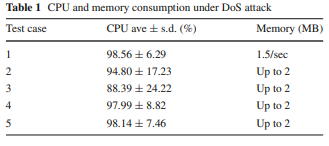
\includegraphics{Apdenix/adiTable.PNG}
    \caption{Table 1 from \cite{adi2017stealthy}}
    \label{fig:my_label}
\end{wrapfigure}
The 2016 study carried out 4 varying investigations to analyse the behaviour of a victim machine when subject to large volume low rate DoS attacks. The researchers used a flood of windows PING and WINDOWS UPDATE frames to Simulate a Low-Rate DoS attack on a server, and demonstrated how legitimate HTTP/2 Flash Crowd could be launched to create a DoS scenario.  The team noted at the time of their 2016 investigation that there was no reported study to ascertain whether or not attack traffic could be concealed in a stealthy manor to appear as legitimate Flashcrowd traffic. The research concluded that the HTTP/2 protocol itself does not restrict the intensity of traffic generated, and that auxiliary mechanisms should be implemented for identifying volumes and patterns of network traffic. (\cite{Adi2016}) Trapathi stated as criticism in his 2018 study that neither the 2015 or 2016 studies completed by Adi's team managed to achieve a completed exhaustion of computational resource (\cite{tripathi2018slow}) Therefore it could be argued that Adi's research did not represent the full effect of a DoS attack, when looking into detail of the results from Adi's research, the figures quoted in Table 1 in the paper by Adi show depletion rates of between 88.39\% to 98.56\% (\cite{Adi2016}). Due to the ineffective depletion of the CPU the majority of his detection methods should be questioned. Erwin Adi himself points out that his methodology could potentially be flawed due to the reduction of resource status that was achieved. Therefore Adi's proposed method for monitoring CPU depletion as a way to detect low rate bandwidth attacks could be fundamentally in-concise. Adi's study was completed on a server with one single website and did not run any other background services for example, email, which would in theory add unpredictable CPU loads and make his detection method difficult to implement.

\begin{wrapfigure}{L}{}
\label{web using h2}
    \centering
    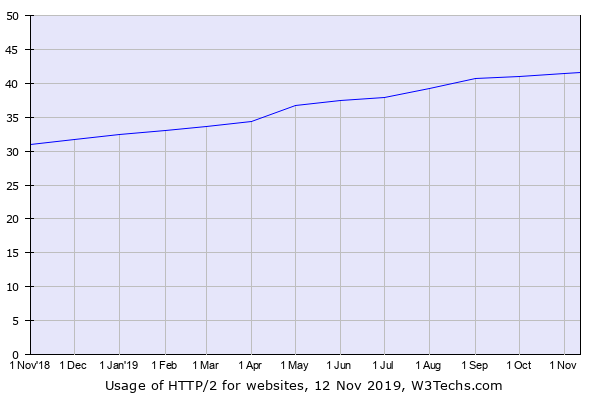
\includegraphics[width=88mm,scale=0.8]{Apdenix/HTTP2SITESgraph.png}
    \caption{Usage of HTTP/2 for Websites, 12 Nov 2019, W3Techs.com}
    \label{web http2}
\end{wrapfigure}
Although Adi's 2016 work looked at HTTP/2 it was noted in their later 2017 paper that 90\% of contemporary web servers up to the date of that study had not yet migrated to HTTP/2 from HTTP/1.x (\cite{adi2017stealthy}) At the time of this paper November 2019, HTTP/2 was used by 41.7\% of the top 10 million websites (\cite{w3techs}), as seen in figure \ref{web http2}. This illuminates the pressing need for research into the assailability of the HTTP/2 protocol and consequent detection methods and fixes. 
 
Tripathi's 2018 study took a sample of websites and attempted to detect Low rate attacks by monitoring benchmarking and measuring the Chi squared (X\textsuperscript{\small2}) differential value between the expected and observed traffic pattern. Tripathi suggests this approach could detect attacks with high accuracy and may lead to further research to assess further HTTP/2 vulnerabilities thus potentially mitigating these threat vectors with fixes. Trapathi indicated that although his detection method for attack traffic was successful; if HTTP/2 traffic data is encrypted it must then be decrypted before submitting traces to the detector. He suggested that this could be easily achieved with the aid of an intercepting proxy before forwarding to the target website responsible for handling HTTP/2 requests. It must be noted that most large companies are utilising this strategy to intercept traffic coming into their local network. (\cite{tripathi2018slow}). 

Adi's 2017 work looked at some of the stealthier approaches that cyber attacks were using in order to bypass current detection methods. Adi and his team set up two models intended to simulate stealthy Low rate DoS attacks which they called 'bots'. The investigation aimed to model attacks whose traffic continually consumed the victims computing resource, while still being stealthy enough to yield some false alarms via the target servers' 'learning' mechanisms. Adi constructed the attack 'bots' with four core factors for experimentation, these were number of threads, number of window\_update, stealthy factor and delay between successive TCP connections. These two sets of Stealth models were tested against regular flash crowd traffic in an effort to differentiate the pattern. The experiment and subsequent analysis was successful in distinguishing a notable difference in the patterns of the number of packets carrying SYN flags per 1-second traffic instance between regular flashcrowd traffic and the simulated stealthy attacks. (\cite{adi2017stealthy}) Since Adi's work there appears to be an implementation of the methodology proposed in their paper. Cloudflare have been able to implement a defence mechanism against a SYN flood attack. The have created a program called 'gatebot' which monitors SYN packet packet requests and attempts to drop malicious SYN packets on the firewall layer (\cite{CFSYN}) the work does not refer to that of Adi's however the cloudflare implementation does appear to use similar concepts. At the  time of writing this seems to be the only documented attempt of blocking SYN attacks.
\section{port scanning}

A port scanner attack is a attack whereby an attacker will send packages of information to different ports on a server to see which ports can be accessed; this may lead them to be able to log into different parts of the server using a brute force approach. Some of the standard ports that are use d in a web server are WWW 80, ftp 21 and nameserver 53 (REF NEEDED). SSH 22. A lot of web hosts and sever owners change the ports for SSH and the ftp however, they may inevertinbly (how spell) leave ports open that are not secure. 
READ https://ieeexplore.ieee.org/stamp/stamp.jsp?tp=&arnumber=6122824
%\subsection{Different types of Port Scanning Attacks}

After reading the literature regarding the various attacks, the types of port scanning attacks can be condensed down to the 5 following categories:
\begin{itemize}
    \item Ping Scan
    \begin{itemize}
        \item The method of ping scanning entails sweeping an entire network block or a single target, to asses if the target is live. It sends an ICMP echo request to the target, and if the response is an ICMP reply, then you know the target is alive. It is becoming increasingly common that ICMP pings are being blocked by firewalls and routers, that this attack method is becoming ever more ineffective.
    \end{itemize}
    \item TCP Half-Open
    \begin{itemize}
        \item This is probably the most common type of port scan. This is a relatively quick scan that can potentially scan thousands of ports per second. It works this way because it does not complete the TCP handshake process that was discussed in section \ref{attack1} of this chapter. It simply sends a packet with the SYN flag set and waits for the SYN-ACK from the target and does not complete the connection. After identifying open ports the attacker may then escalate this probe with a further attack, for example a brute force attack against an open port.
    \end{itemize} 
    \item TCP Connect
    \begin{itemize}
        \item This port scanning technique is essentially the same as the TCP Half-Open scan, however, instead of leaving the target hanging, the port scanner completes the TCP connection. It must be noted that this method of scanning created a lot of noise that can easily be detected as malicious activity, hence this particular scan is less stealthy and less popular than other methods.
    \end{itemize}
    \item UDP
    \begin{itemize}
        \item Essentially similar to the Ping scan the UDP scans are most common to detect DNS, SNMP and DHCP services. UDP scans work by sending a packet, which is usually empty. If the target responds with an ICMP unreachable error, the attacker can assume that that port is closed. If it responds with an ICMP unreachable error packet with other codes, the packet is considered filtered. If no response is received at all, the port is considered open or filtered. This is a particularly unreliable and sluggish method of scanning as they may be waiting for a packet that may never come. An attacker may have to send numerous packets then wait to make sure a port is considered open or filtered. The problem with using any communication with UDP is that it is unreliable – it has no way of creating an established connection or synchronizing the packets like TCP does. For this reason, UDP scans are typically slow and unreliable. The attacker needs to wait for a packet that may never come, and has no real way of telling if the packet even got to the destination in the first place. An attacker may have to send numerous packets then wait to make sure a port is considered open or filtered.
    \end{itemize}
    \item Stealth Scanning
    \begin{itemize}
        \item These scan types are known as stealth scanning because the packets are engineered in such a way that the attacker is  to induce some type of response from the target without actually going through the handshaking process and establishing a connection. In general these types of scans are elusive to detection methods because they are unlikely to appear in logs and are some of the most minimal port scanning techniques available. The weakness of this method is that because of the way that Microsoft implements the TCP/IP stack, all ports will be considered closed, hence making the number of vulnerable target devices much smaller. If the attacker does receive an open port, they will automatically know that the target is using an alternate operating system to Microsoft Windows.
    \end{itemize}
\end{itemize}






\subsection{Attack Detection Techniques}

Due to the generalised mechanics of the different types of Scanning attacks that have been revealed in the previous section, port scanning should be relatively easy to detect in most cases. Unlike low bandwidth attacks, there is a long history of detailed detection methods for port scanning. The evolution of these techniques will be discussed in the review of the following literature.

\subsection{Snort}

An early port scanning detection technique was Snort. It was created as an open source network intrusion detection based on Libpcap. The detector, used in Staniford's work, attempts to look for (x) TCP or UDP packets sent to any number of ports from a single source in (Y) seconds and assesses the behaviours of this activity for notable malicious scanning characteristics (\cite{staniford2002practical}). The Snort program also looks for single TCP packets that are not used in genuine TCP operations which may have unusual TCP flag settings or no flags set at all. There are several drawbacks of this program. Firstly it is unable to detect scans coming from multiple hosts. The second weakness is that the threshold is determined  and evaluated by using a static combination of user specific data; this method is easy to deceive due to the fact that the Y value has to be set high enough so that there are very few false positives. Therefore, incoming attacks can avoid detection relatively easily, if the attacker increases the time between each successive packet.

A study conducted by \citeauthor{laroche2009evolving} in \citeyear{laroche2009evolving}, attempted to create a stealthy scanning approach to test the limitations of the Snort detection program. A mimicry model was created using a type of computer learning defined as Genetic Programming (GP). Stealthy portscan models were generated and launched with valid attributes (i.e valid TCP/IP packets). The researchers demonstrated that they successfully applied Genetic programming and produced a stealthy mechanism of port scanning that was able to fool the Snort system (\cite{laroche2009evolving}). This research shows that snort was not a reliable way of detecting portscan attacks due to the evolving techniques that can be implemented by attackers, however, Staniford in his 2002 paper proposed a second technique called Spice.
 
\subsection{Spice}
 
Spice is made up of two parts, an anomaly sensor and a correlator component. The researchers noted that saving information about packets would have a detrimental effect on performance, hence they took the approach of storing the details of more likely candidates for malicious activity for longer. The anomaly sensor looked at the suspicious features of the following; header fields, source IP, destination IP, source port, destination port, protocol and protocol flags. The researchers used a Bayesian Network statistical approach to assess the probability of anomalous entries in order to score events in their likelihood of being malicious port scan attacks. Finally, a heuristic analysis is carried out as part of the correlation process where the data is evaluated. It was noted by the research team that a limitation of the Spice detection method is that port scanning attacks that are similar in nature to normal traffic could bypass the anomaly detector. Thus, resulting in a stealthy scan attack not being identified as a threat(\cite{staniford2002practical}); this in turn makes Spice a fundamentally flawed detection method due to the evolving nature of port scan attacks, and the stealth scans discussed in the prior section.


\subsection{Stealth Attacks}

\citeauthor{kim2008slow} defined stealth scans as a technique that avoided Intrusion detection and prevention systems. Intrusion detection systems are detection and monitoring tools that don't take action on their own. They also suggest that stealth methodology has evolved into the setting of flags and the interval between scans in order to appear as normal traffic (\cite{kim2008slow}). The researchers went on to propose a novel detection method using fuzzy logic in order to categorise the architecture and periodicity of incoming port traffic into 3 distinct classifications; this was done by establishing a scoring system in an effort to indicate the potential of each request as being a malicious scan attack. The researchers went on to propose a managing mechanism in order to filter the 3 traffic types in terms of bandwidth allowance using 'stepwise strategies'. It should be noted that in their approaches the authors suggested some drawbacks with this methodology, appreciating that there is no standard of judgement about slow port scan attacks, and there is always a degree of uncertainty while using this technique to detect slow port scans.

All of the research within the field of port scanning is particularly similar in nature, this may be due to the common feature nature of port scan attacks in general. Whether via a heuristic analysis, or even the artificial intelligence methodologies discussed, a degree of uncertainty remains with each system which poses a risk for error in identification. The fact remains that at least some genuine traffic will be blocked due to the 'generalised property rules' that are applied at the managing stage of each system. The papers suggest that there is need for a human factor in judgement within the filtering process, in order to effect confidence in blocking features. In conclusion, although the mitigation techniques presented in this section are impressive and enlightening, they should perhaps be implemented in an advisory capacity rather than as an exclusive method of detection and mitigation.

%\quickwordcount{}
\section{conclusion}
\chapter{Review of current detection methods for high bandwidth attacks}
%!TeX root=Dissertation.tex

\section*{Introduction}
This chapter will look at the various types of high bandwidth attacks that can occur in particular looking at DDOS attacks. A high rate bandwidth attack is essentially a malicious attempt to over run a server with an immense amount of traffic in attempt to disrupt its functionality. Unlike the portscan and low rate attacks mentioned in the prior chapter, the high rate attack sends multitudes of requests all at the same time. It is important to note that the effects delivered from these types of attacks are the most devastating of the three types of attacks that have been discussed to this point. A successful attack can essentially lockdown a targeted website that is unprotected for the duration of the attackers strategized window of service denial. 
%!TeX root=Dissertation.tex

\section{DDOS attacks} \label{attack2}
%https://reader.elsevier.com/reader/sd/pii/S0140366417303791?token=098B9C0758047352DF30300332E273B21DB9C488D1FE2D089522058BA6FD67DC86B8FC286ABBA0C30D94E897E4808B93

High-bandwidth attacks can have serious implications for businesses as they can take a website offline, therefore, the early detection of high-bandwidth DDoS attacks is crucial. An example of prompt mitigation of a bandwidth DDoS attack can be seen in the Githhub Case 2018; where by a 1.3 Tps high-bandwidth attack was launched against Githhub bringing services to a stop for 9 minutes. \cite{Githhubattacks} This case shows how important it is to have prompt detection and mitigation of high rate DDoS attacks. Due to the commercial nature of providing mitigation technologies for high-bandwidth attacks, there is very little publicly available material on the architecture and design of defence mechanisms. However, some rudimentary detection and mitigation techniques have been proposed publicly by academics. 

In the modern world businesses will take the networking approach of either using a reverse proxy via a provider such as cloudflare, or by the use of in house networking mechanics such as SDN or NFV. The majority of the papers found while researching high bandwidth attacks are looking into detection methodology while using SDN networking. SDN networking is more important now due to the adaptation of the cloud by using SDN networking (FIND LOST PAPER --- LINK ABOVE). The cloud allows the business to automatically scale the resources on a server automatically to deal with peaks in traffic. However, if an attack is not managed properly the server will continue to scale therefore increasing cost for the organisation. 

Haopei Wang notes in 2015, when the emergence of SDN networking was relatively new, that SDN abstracts the physical layer from the hardware layer therefore the control of the network is done at the software; this therefore leads to a more fine grained control of the network and opens up the opportunity for new defence mechanisms. The team developed a DDoS identifying and mitigation process that they named FLOODGUARD. The process involves a two stage saturation mitigation technique involving a Proactive flow rule analyzer and a packet migration module. Through a comprehensive detection algorithm at the migration agent, looking at Memory depletion and rate of packet\_in messages, malign traffic is separated from genuine traffic and mitigated using handling dynamics. (check d. handling dynamics)


The most recent paper available was written by \citeauthor{ahalawat2019entropy} He assessed the use of SDN networking and theorised that entropy could be used as a measurement of randomness in an effort to detect DDoS traffic. A mitigation technique was introduced by limiting the rate of packet flow allowed to flow to the switch, while in turn, Attack control plane bandwidth is prevented by limiting the inflow rate to the controller.  The team concluded that SDN networks seemed to be in particular most vulnerable to DDoS attacks that flooded the network with UDP packets. The researchers noticed that this mitigation technique had the ability to be implemented much earlier than some other techniques that had been previously researched and developed. It was also successful in restoring the use of services to 'normal traffic.' (\cite{ahalawat2019entropy}). Another study to ustilize entropy as an early detection and mitigation teqhnique took place in \citeyear{kumar2018safety}  (\cite{kumar2018safety}) 

The software for this dissertation will not have a primary focus on focusing on high rate bandwidth attacks, due to the fact that they require immediate mitigation to avoid disruption to web services. Also as discussed earlier in this section, detection and mitigation tend to be handled at a control plane phase through networking, or at the filter stage if the website has an independent CDN. Some of the methodology for defence and case studies through industry will be discussed in the next section.
%%!TeX root=Dissertation.tex

\section{Other common attacks} \label{attack3}
A highly common attack on Wordpress websites is a brute force login attack. These attacks are relatively easy to do as they only involve trying to guess user names and passwords. There are solutions such as Wordfence that will detect and block these attacks, however, there is an inherent weakness of this whereby there is a chance that there is an attack so large that it will become powerful enough to take down the server. Solutions already exist for this type of attack, therefore my software only needs to look at whether a user is trying to access the login page, and factor this into the risk for an IP address.

An SQL injection attack is a common form of attack as most websites use an SQL database in some capacity. The inherent attack risk with any SQL application, particularly websites is usually people injecting malicious code into text boxes that are not checked before being sent to the database, therefore, allowing them to run in the database undetected.
%https://www.theregister.co.uk/2015/07/10/spamhaus_ddos_teen_sentenced/ 
\chapter{Human factors}\label{Human factors}
%!TeX root=Dissertation.tex

\section*{Introduction}
This chapter will look at the requirements of the software in relation to the \nameref{Moscow} ( apdendix 
\ref{Moscow})

For the purpose of clarity the decision was made to group sections of the MOSCOW for justification due to the way in which they interact with one another, within the body of the software.
\section{Justification}

\subsection*{Detect attacks}
The primary target of the software shall be the detection of potentially malicious IP addresses. By looking at different threat vectors contained within the log files, for example; the frequency of which an IP address accesses the website, or the type of data these access events are attempting to acquire (the log in pages). The software must have the ability to assess and differentiate between similar IP activity (See section on the \nameref{Learning loop and known IPs} for details), an example of the type of attack that could be detected is shown in appendix \ref{Log file example} below.

\subsection*{Analyis of Log files}
Alongside the primary goal of the research application is the ability to analyse website access logs; to address this goal the software needs to be able to read in data. Due to the fact that the data files are not in a easily interpreted format the software should be able to handle the input of varying amounts of data. The data can be represented in a text document, therefore, the software should be able to read a text file quickly and easily. Due to the complexity of the data as explained in this section, the decision was made to allow a flexible amount of data to be uploaded to the system. Due to the fact that this software is not running on a server, the limitations of recording too much data, and hence affecting performance levels, is removed; This was reinforced when researching \cite{staniford2002practical}, and their team noted that they theorised a detrimental performance effect when accumulating too much data regarding incoming packets; this is also why the program needs to run efficiently.

\subsubsection*{File reading ability}
The reason that the software is written using the extended Apache log format is that this data is easily accessible for the authors of this report. To keep the functionality of the overall architecture simple, the decision was taken to use one single format for file reading in order to better assess the validity of the software. (reference Adi studies, to back up the BS, using one PC servers) Apache was the most popular web server at the time of this research and due to the fact that lightspeed is using similar technology and is also Apache compatible, this means that using apache as a webserver is justifiable as between lightspeed and apache, 58.35\% of the market share server type coverage is Apache compatible. (see figure \ref{the market share of Apache web servers})
All servers show their log data using different systems of segregated data. The software should ideally be able to read all the different log files. The ability to do so could be implemented at a later date if required. 
\begin{figure}[H] \label{the market share of Apache web servers}
    \centering
    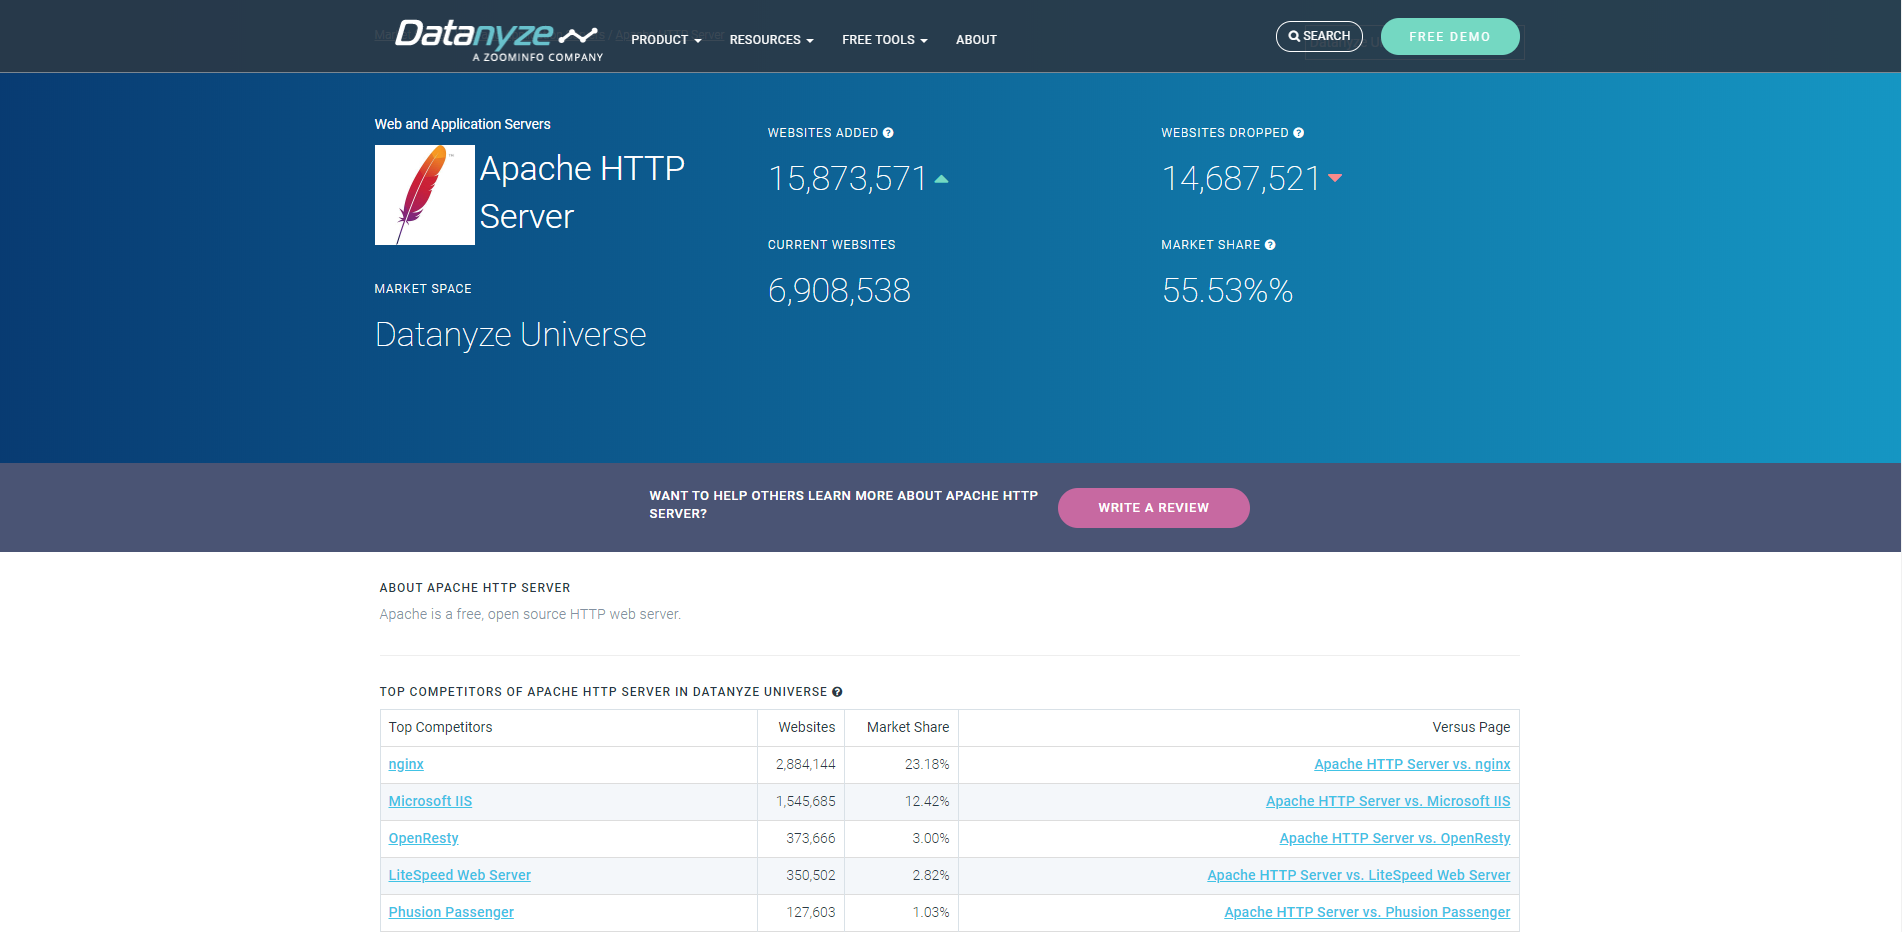
\includegraphics[width=88mm,scale=0.8]{Apdenix/MarketshareApache.PNG}
    \caption{the market share of Apache web servers \cite{Apache}}
    \label{the market share of Apache web servers}
\end{figure}
\subsection*{Learning loop and known IPs} \label{Learning loop and known IP's}

The learning loop described in the MOSCOW shall be fairly basic and the loop will have two primary functions. The first is simply the ability to distinguish malicious IP addresses from the collated data. The secondary function is to identify and flag up potential candidates from the IP collection that could potentially be search engine bots. These requests may have many similarities in architecture. The IP of a bot could have different address patterns, even if sent from the same host, and these bot IPs may change periodically. This would require a larger amount of inputting of data, therefore, it may be easier to have a community driven approach. Due to the potential for abuse such as a hacker adding their IP to the proven bot list, there is a secondary requirement that an overseer approves all the good bots manually.

\subsection*{Database}
For the justification purposes of database type, the different types of database shall be assessed in this section. The first database that has been considered is a NoSQL database namely, MongoDB. MongoDB is a document-oriented database and is currently the most popular NoSQL database at the time of this research.  MongoDB makes it easy to access documents by indexing, hence, it provides a fast query response. A great advantage of MongoDB is that it is a horizontally scalable database, and when you have to handle a large amount of data, it is possible to distribute it to several machines (\cite{MongoDB5}). During the development phase there shall only be one user machine. During the implementation of the software, however, the server will scale, this is an appropriate feature supporting the justification of MongoDB. MongoDB does not support joins in the way a relational database would; it may slow execution and affect performance (\cite{MongoDBComp})) This disadvantage may have a detrimental effect on the operation of the software, as the data will need to be stored on multiple tables. MongoDB stores key names for each value pair. Also, due to 'no functionality of joins', there is a data redundancy trend. This may result in increasing unnecessary usage of memory and once again is a limitation that may effect the software.

Another alternative database type for the software could be an SQL. An advantage of this database is that by using SQL queries, the user can quickly and efficiently retrieve a large number of records from a database. This would have a positive effect on the processing speed while running the software. In the standard SQL, it is very easy to manage the database system. It does not require a substantial amount of code to manage the database system. This will help to keep the code for the database neat and tidy, and the code required for accessing the database will also be kept similarly trim and orderly. SQL can be used in laptops, PCs, servers and even some mobile phones, which will aid in the development of the software through multiple access vectors (\cite{JavaTPoint}). Microsoft access could be used to develop this software as it is a popular SQL database that can easily be run on a computer with Java integration. If this approach is selected as the database candidate, it would also present a key supporting justification for the utilization of java coding, this will be discussed later in the section on the \nameref{Language} for details.  


\subsection*{API }
A lot of the API's may be able to provide data to the software for example, abuse IP's and GOIP's. Free API's are available from many data base hosts that can identify abuse IP's for example (https://www.abuseipdb.com/). This API could be embedded in the software to assist in identifying malicious IP's. An example of an integration technique that is not classified as an API yet still aids in the data provided at the GOIP level is Geolite2. This program helps to locate and pinpoint the coordinates of an incoming IP address hence assists in the identification of malicious IP's. The overall decision to not use API's was made to keep the data that is collected by the software secure. If the choice was made to allow for API's it very well could be the case that an attacker may realise that they have been discovered and this may effect the overall analysis of the software.

\subsection*{Language} \label{Language}
Many languages were considered including Python, C, PHP and Java. Java is architecturally neutral and would work particularly well for the project as it can be run on any machine. As many users will be utilizing the finished software on various platforms, the use of Java would be advantageous. The use of C as a language was also considered. C is a language that runs on many Unix systems on which most servers run, however, in the modern world most website owners do not necessarily have access to the server that their site is hosted on. Another reason for standing against the utilisation of C as a language is that this language may not be appropriate for the development of a user interface that will be required as a vital component of the software. Python was considered as an alternative code for the project, however, the main issue that was discovered with python was its limitations with database access. If compared to popular technologies like JDBC and ODBC, the Python database access layer is found to be somewhat underdeveloped and primitive. Due to the proposed architecture of the software, python would not be a suitable language, as fluid database communication is integral to the project. Finally, PHP was considered as a language for the project because the software could be implemented as a web based application. Unfortunately, this approach may have given the attackers access to the data as it is open sourced. This would defeat the overall objective of the project and the software.  

\subsection*{Data Controller}
The decision was made to limit the influence that the computer has on the mitigation of attacks. Many of the papers mentioned in the literature review applied some kind of machine learning or formulaic protocol to ringfence potential malicious attacks and mitigate them. In the majority of the papers looked at there was a margin of error, or degree of uncertainty with these results due to the methodology in their approach. Due to this, the decision was made to enrol a data assessor to the process in order to filter out the IPs that the software had picked up as potentially malicious. This human approach will allow with 100\% certainty that only malicious IPs will be blocked, reported or otherwise actioned. 
\chapter{Tools, packages and Requirements Specifications}
%!TeX root=Dissertation.tex

\section*{Introduction}
In previous chapters the literature around detection of attacks has been reviewed and critiqued. In the following chapter a novel approach will be discussed and tested. This chapter will look at the requirements of the software in relation to the \nameref{Moscow} (appendix \ref{Moscow}). Some of the requirements outlined in the \nameref{Moscow} will be discussed together rather than as individuals to provide a clear overview of this software.
\section{Justification}

\subsection*{Detect attacks}
The primary target of the software shall be the detection of potentially malicious IP addresses. By looking at different threat vectors contained within the log files, for example; the frequency of which an IP address accesses the website, or the type of data these access events are attempting to acquire (the log in pages). The software must have the ability to assess and differentiate between similar IP activity (See section on the \nameref{Learning loop and known IPs} for details), an example of the type of attack that could be detected is shown in appendix \ref{Log file example} below.

\subsection*{Analyis of Log files}
Alongside the primary goal of the research application is the ability to analyse website access logs; to address this goal the software needs to be able to read in data. Due to the fact that the data files are not in a easily interpreted format the software should be able to handle the input of varying amounts of data. The data can be represented in a text document, therefore, the software should be able to read a text file quickly and easily. Due to the complexity of the data as explained in this section, the decision was made to allow a flexible amount of data to be uploaded to the system. Due to the fact that this software is not running on a server, the limitations of recording too much data, and hence affecting performance levels, is removed; This was reinforced when researching \cite{staniford2002practical}, and their team noted that they theorised a detrimental performance effect when accumulating too much data regarding incoming packets; this is also why the program needs to run efficiently.

\subsubsection*{File reading ability}
The reason that the software is written using the extended Apache log format is that this data is easily accessible for the authors of this report. To keep the functionality of the overall architecture simple, the decision was taken to use one single format for file reading in order to better assess the validity of the software. (reference Adi studies, to back up the BS, using one PC servers) Apache was the most popular web server at the time of this research and due to the fact that lightspeed is using similar technology and is also Apache compatible, this means that using apache as a webserver is justifiable as between lightspeed and apache, 58.35\% of the market share server type coverage is Apache compatible. (see figure \ref{the market share of Apache web servers})
All servers show their log data using different systems of segregated data. The software should ideally be able to read all the different log files. The ability to do so could be implemented at a later date if required. 
\begin{figure}[H] \label{the market share of Apache web servers}
    \centering
    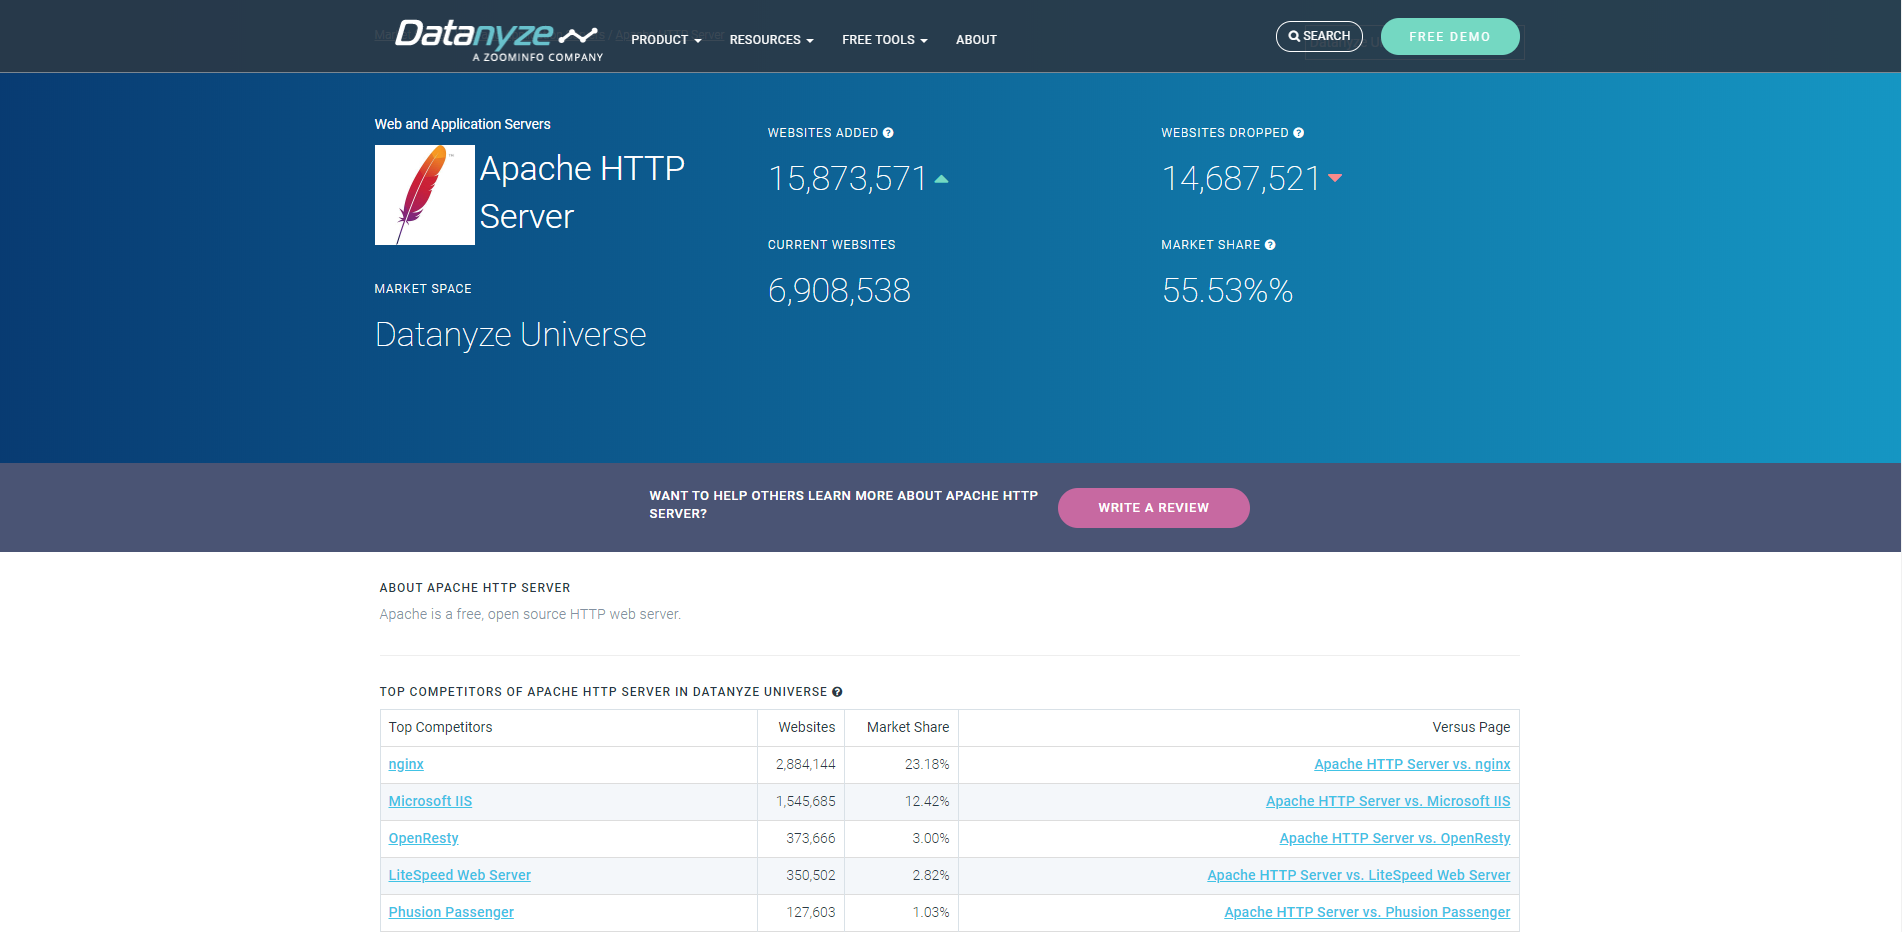
\includegraphics[width=88mm,scale=0.8]{Apdenix/MarketshareApache.PNG}
    \caption{the market share of Apache web servers \cite{Apache}}
    \label{the market share of Apache web servers}
\end{figure}
\subsection*{Learning loop and known IPs} \label{Learning loop and known IP's}

The learning loop described in the MOSCOW shall be fairly basic and the loop will have two primary functions. The first is simply the ability to distinguish malicious IP addresses from the collated data. The secondary function is to identify and flag up potential candidates from the IP collection that could potentially be search engine bots. These requests may have many similarities in architecture. The IP of a bot could have different address patterns, even if sent from the same host, and these bot IPs may change periodically. This would require a larger amount of inputting of data, therefore, it may be easier to have a community driven approach. Due to the potential for abuse such as a hacker adding their IP to the proven bot list, there is a secondary requirement that an overseer approves all the good bots manually.

\subsection*{Database}
For the justification purposes of database type, the different types of database shall be assessed in this section. The first database that has been considered is a NoSQL database namely, MongoDB. MongoDB is a document-oriented database and is currently the most popular NoSQL database at the time of this research.  MongoDB makes it easy to access documents by indexing, hence, it provides a fast query response. A great advantage of MongoDB is that it is a horizontally scalable database, and when you have to handle a large amount of data, it is possible to distribute it to several machines (\cite{MongoDB5}). During the development phase there shall only be one user machine. During the implementation of the software, however, the server will scale, this is an appropriate feature supporting the justification of MongoDB. MongoDB does not support joins in the way a relational database would; it may slow execution and affect performance (\cite{MongoDBComp})) This disadvantage may have a detrimental effect on the operation of the software, as the data will need to be stored on multiple tables. MongoDB stores key names for each value pair. Also, due to 'no functionality of joins', there is a data redundancy trend. This may result in increasing unnecessary usage of memory and once again is a limitation that may effect the software.

Another alternative database type for the software could be an SQL. An advantage of this database is that by using SQL queries, the user can quickly and efficiently retrieve a large number of records from a database. This would have a positive effect on the processing speed while running the software. In the standard SQL, it is very easy to manage the database system. It does not require a substantial amount of code to manage the database system. This will help to keep the code for the database neat and tidy, and the code required for accessing the database will also be kept similarly trim and orderly. SQL can be used in laptops, PCs, servers and even some mobile phones, which will aid in the development of the software through multiple access vectors (\cite{JavaTPoint}). Microsoft access could be used to develop this software as it is a popular SQL database that can easily be run on a computer with Java integration. If this approach is selected as the database candidate, it would also present a key supporting justification for the utilization of java coding, this will be discussed later in the section on the \nameref{Language} for details.  


\subsection*{API }
A lot of the API's may be able to provide data to the software for example, abuse IP's and GOIP's. Free API's are available from many data base hosts that can identify abuse IP's for example (https://www.abuseipdb.com/). This API could be embedded in the software to assist in identifying malicious IP's. An example of an integration technique that is not classified as an API yet still aids in the data provided at the GOIP level is Geolite2. This program helps to locate and pinpoint the coordinates of an incoming IP address hence assists in the identification of malicious IP's. The overall decision to not use API's was made to keep the data that is collected by the software secure. If the choice was made to allow for API's it very well could be the case that an attacker may realise that they have been discovered and this may effect the overall analysis of the software.

\subsection*{Language} \label{Language}
Many languages were considered including Python, C, PHP and Java. Java is architecturally neutral and would work particularly well for the project as it can be run on any machine. As many users will be utilizing the finished software on various platforms, the use of Java would be advantageous. The use of C as a language was also considered. C is a language that runs on many Unix systems on which most servers run, however, in the modern world most website owners do not necessarily have access to the server that their site is hosted on. Another reason for standing against the utilisation of C as a language is that this language may not be appropriate for the development of a user interface that will be required as a vital component of the software. Python was considered as an alternative code for the project, however, the main issue that was discovered with python was its limitations with database access. If compared to popular technologies like JDBC and ODBC, the Python database access layer is found to be somewhat underdeveloped and primitive. Due to the proposed architecture of the software, python would not be a suitable language, as fluid database communication is integral to the project. Finally, PHP was considered as a language for the project because the software could be implemented as a web based application. Unfortunately, this approach may have given the attackers access to the data as it is open sourced. This would defeat the overall objective of the project and the software.  

\subsection*{Data Controller}
The decision was made to limit the influence that the computer has on the mitigation of attacks. Many of the papers mentioned in the literature review applied some kind of machine learning or formulaic protocol to ringfence potential malicious attacks and mitigate them. In the majority of the papers looked at there was a margin of error, or degree of uncertainty with these results due to the methodology in their approach. Due to this, the decision was made to enrol a data assessor to the process in order to filter out the IPs that the software had picked up as potentially malicious. This human approach will allow with 100\% certainty that only malicious IPs will be blocked, reported or otherwise actioned.  \label{Errorcodes}
\chapter{Design and Implementation}
*Note to self, Critisism based around not using webservers with IIS. This would have given further details into Request Errors and would have helped to disclude some 'over-banding' principals in risk factors. For example see 400 errors. 
\chapter{Testing}
\section{ui testing}

Although the UI is not a major part of the project, it will still be important to check that the UI implemented the functionality required in the system therefore, the UI was tested as the software was being built. All components of the the UI were functional as they were implemented however, when looking back over the software it was found there were some errors in the spelling of words and some text needed rewording to aid the user experience. 

it was noted that the button that is needed to read the file, although this was stated on the button the button is not very clear in how to display the data. It would have been useful to make this button clearer in some way however due to time constraints in this project this would require extensive reworking of the program which time constraints did not allow. By adding the words \textit{start here} to the button; this made the button bigger and provided clear instructions on how to start the process.
\section{Test Plan}

Although the usability of the software is important as outlined in section \ref{UI Theory} due to the scale of testing that would be needed and recrutmet issues outined in \cite{ben2015effects} it was decided that it would be better "proving" if the formula was able to identify and classify attack traffic. 

4 IP's shall be chosen one will be a high volume IP, to see if the occurrences part of the formula works.
\section{Evaluating the Formula}
In this section, the formula, that was discussed in chapter 6, shall be evaluated in order to assess its ability to detect malicious trends in traffic. This thesis shall then go on to evaluate the UI in terms of its functionality, by doing so, the hypotheses raised in the prior chapter shall be evaluated.

Three websites were assessed over a one month period and log file data was collected from each site throughout this period. The data captured from the website logs was taken in late January and early February 2020. It should be noted that two variables were chosen in order to display the data and results in a graphical summary. These represent the risk rating versus the occurrences of the IP. The risk rating is an obvious choice for a variable due to the fact that it is the key focus of the software and the proving factor for the majority of the hypothesis. The occurrences were chosen as the second variable due to the fact that they were the aspect that were given the highest weight rating in terms of risk. If the researcher were to look at the requests and responses, they would need to log every occurrence of each response code, which would be difficult to display in the form of a graph.



After looking at the graphical display of data, as it can be seen in appendix 
\ref{Graph data} it was clear that a trend exists between extreme levels of occurrences and a higher risk rating. Six out of out of nine IP addresses with occurrence counts of over 1000, fall within the highest 0.3\% of risk ratings. It should be noted that a huge number of IP addresses seem to fall into the categorisation of low risk rating. 99.45\% of readings fall into the banding of a risk rating of less than 10. For the purposes of testing, in order to analyse the formula in detail, the 10\% from the database that would normally contribute to the score was ignored, therefore if an IP got 100\% in testing then this would equate to 90\% overall.

In order to evaluate the elements of these results it was decided to take some of the IP instances with the highest risk related factors and attempt to diagnose them as malicious or genuine. The decision was also made to look at some of the more anomalous readings, particularly those that fall far outside of the 'trend-line'. These values tend to be those with particularly high occurrence ratings and yet with low risk factor readings, or those with large risk factor ratings and particularly low occurrence ratings. The architecture of these traffic occurrences shall be evaluated individually in order to make conclusions regarding whether or not they display any signs of being a malicious entity.

\subsection{Detailed look at IPs }
In order to further assess the capabilities of the formula. Seven IPs shall now be cross referenced with the data held on abuseipdb. As discussed, these IP's were those displaying the highest risk rating score, and also those falling far from the 'trend-line' on the data set. It is anticipated that this will show the ability of the formula in detecting true attacks.

\subsection*{194.61.24.46}

This IP address originated from the Netherlands. After corresponding with the abuseipdb it was found that this IP has been reported a staggering 1104 times due to malicious trending visits to other websites. After looking deeper into the raw data, it was clear to see that the chains of 403 and 404 responses were patterned in a systematic repeating cycle; thus it is is fair to conclude that this is a malicious entity with bot like features. The software was able to flag this and gave the IP a risk related scoring of 100/100.  

\subsection*{209.124.66.6}

This IP address originated from the UK, this would be a 'best fit' source location to signify a level of inherent trust, due to the UK based websites used in testing. However, when consulting with abuseipdb it becomes apparent that this IP address has been reported for malicious activity 14 times. The formula inferred a risk related rating of 100/100 for this IP source, and the IP was the source of 9134 requests from one particular website within the test window. The responses allocated to the IP GET requests across the test window were made up of chains of 301 and 404 errors. While a 301 response, indicating a redirection for a URL has not been given a risk related factor, in this instance, the continued appearance of these responses are particularly indicative of a potential threat. Along with the 301 responses, a huge string of repeated and systematic 404 errors were returned to the IP source. Altogether it is clear that this IP is the source of malicious traffic, and the formula was correct in applying a maximum risk related flag.

\subsection*{86.175.235.192}

This IP originated in the UK, and it would be appropriate to discuss the features of the IP address and why it may not be malicious. This IP was allocated a risk rating of 100/100, however it is believed that this was a false alert. Firstly this IP has never been reported or raised as a candidate for malicious activity on abuseipdb. The request pattern of the IP address appears to be random in nature, therefore, this does not indicate a bot, as this would be in a systematic pattern. In addition to this, there are a number of 200 response codes, therefore, indicating that some of the requests are legitimate and only some of them are not. An explanation of the pattern may be that the website to which this data belongs was under development; this would generate errors during the testing period. It may therefore be reasonable to predict that this is administration activity. If this is the case it raises a concern regarding the possibility of a false alert being generated by administrators during the building and testing phases of website design. If the rationale that has been adopted to explain this anomaly is correct, it raises the importance of having a human moderator in the detection methodology. Any experienced user would be able to identify their own IP address and de-escalate this false flag.

\subsection*{35.187.118.51}

This IP had the highest number of occurrences within the testing period. Its risk factor hit the maximum score of 100/100. After further study of the data set, it appeared that this IP had made contact with a single website an astonishing 800 times per day, during the period of data collection. After cross referencing with abuseipdb it was found that this IP had previously been reported as a source of malicious activity. The source of the IP was identified as the USA, therefore has a risk related country of origin factor. The raw data within the log files shows a huge string of repeated 403 response codes. This is indicative of malicious activity due to repeated, bot like, attempts to access forbidden pages. It is therefore concluded that this is almost certainly a malicious IP due to the repetition of unauthorised attempts. It is clear that the software was correct in its assessment that this was a high risk candidate.
\subsection{Anomalies in the Data}
\subsection*{192.173.3.114} 

This IP was randomly chosen to be marked as a BOT with the name of "Test"; this was done in order to check whether or not this feature of the software to detect known bots worked efficiently. This IP was marked with a risk factor of 0/100 which supports the conclusion that the software has the ability to detect functional benign bots. When looking on AbuseIPDB, it would appear that this IP address belongs to the University of Northumbria. Therefore, in response to the purpose of testing, it was able to show the ability of the software to detect bots that are known and flagged as such on the database.

\subsection*{108.162.220.175}

This IP originated from the USA. It was allocated a risk score of 6.46/100 through the formula, yet had a particularly large number of occurrences during the data capture. After exploring the raw data it appears that this is an unflagged bot for a service that monitors the 'up-times' of websites. The GET requests generated a multitude of 200 responses which as discussed in prior chapters help to diminish risk related scoring. If flagged properly as a 'good bot', this IP would have been given a risk score of zero. The instance clearly illustrates that particularly high numbers of IP requests within a time frame do not always lead to a high risk related flag. 'Good' or 'genuine' behaviour is credited through the software and leads to a low risk rating despite the weight of the request instances. The software concluded that this IP was a low risk visitor.

\subsection*{63.143.42.250}

This particular IP originated in the USA. At the time of testing the database held on Abuseipdb it was found to have been reported 14 times previously for malicious trending activity. This IP made contact with one particular website during the testing capture 1173 times. After opening the raw Data, it became apparent that this source was a another genuine bot for an 'up-time' website. After looking deeper into the reports on the Abuseipdb website it would appear that the reports were automatically generated by the sites via automated code parameters. Due to the chains of 200 responses a suitably low risk factor rating was issued by the software for this IP, scoring 5/100. This particular log file was instrumental in showcasing the ability of the software to down rate a previously unlisted 'good bot'. Once again, this scenario also shows the usefulness of a human moderator within the detection methodology. The ability of a moderator to use context and rationale within Abuseipdb helped to assess the benign nature of this bot-like activity.

\subsection{Summary}

It is clear from the evaluation of the formula that it is working correctly. Although some false alerts were generated, these cases were identified in essence by the researcher. This action simulates the comparable actions that a potential human moderator could take as the overall system for identification of threats had intended.
%MUST CHECK IF WE NOTED THAT WE HAVE SPOKEN ABOUT THE  10% PART OF THE FORMULA BEING TREAT AS 10/10 FOR THREAT LEVEL DURING TESTING.
\section{Data not included in the Formula}

The formula as previously shown is able to detect attacks with a fairly high degree of accuracy however, during the testing it became apparent that some data was not taken into account. The protocol used for the request; this could have been added to indicate whether the connection was secure due to the fact the HTTP2 only works on a secure connection therefore, this could have been used as an indicator of how secure the request was and maybe increase the risk if HTTP1 was used and detracted a HTTP2 was used. It could however be argued that more risk factor could have been given to HTTP2 due to the fact that \cite{tripathi2018slow} pointed out that HTTP2 had more threat vectors; due to this uncertainty it was decided it was better to leave the protocol out of the formula. 

Due to the time constraints on this project, the time of day of the traffic was not taken into account; this was because to accurately use this, the local time of the IP address would have needed to be calculated and then a further risk factor plan is required. however, due to the 24 hour nature of the internet this would be difficult to apply risk to.

.We did not look at HTTP1/HTTP2 
.We did not look at the time of day of the requests
.we did not look at 301 error 302, 402
.
\chapter{conclusions}
\section{Evaluated Hypotheses}

In order to make a complete analysis of the formula and software it would be good practise to review the three main hypotheses.  

Firstly, it was hypothesised that the process of collecting log files will be an efficient way of collecting data in terms of space and computational resource. It is believed that this particular hypothesis was answered simply by building a system that uses only log file data. This data is automatically collected by websites and does not generate any additional computational activity. The data is relatively easy to store and takes up very little space. This hypothesis has been addressed to satisfy the criteria, as outlined in the requirements specification.

The second hypothesis is the prediction that there is sufficient data within the log files to diagnose with a degree of certainty, potentially malicious IP traffic patterns by looking at the characteristics of each instance. This hypothesis was satisfied, as the evaluation of IP addresses that had been flagged by the formula as high risk, were concluded to be malicious by a human analyst in chapter 7.  

It was finally hypothesised that by by using a human moderator in combination with a formulaic detection system, that more malicious traffic will be correctly identified and less genuine traffic will be misidentified. During the evaluation of high risk scoring IP instances in Chapter 7, several falsely flagged entities were raised as malicious by the formula. The analyst was able to look into the log files and in each case apply logic to assess each instance on its own merits, then conclude that these high risk candidates were not malicious. This in turn supports the hypothesis, as without the human moderator, high risk candidates would otherwise remain assessed as malicious traffic instances and in turn generate errors.  


\section{Evaluation of Product}

In general the software was able to pick up instances of malign activity that make contact with websites. There were very few false alerts and the majority of genuine network traffic was identified as benign. The few false alerts that made it through the detection system would be assessed and deescalated by the human moderator.

Although some elements of the user interface suffered from computational latency, the data was accessed and presented efficiently from the log files. It was clear to see that the software had the ability to detect malign activity with a good degree of accuracy. During the process of coding it was decided to use clearly labeled variables within the code. This was a particularly intuitive move as it now allows these variables to be tweaked for future patching and testing of the integral formula. 

The way in which the code was implemented was well structured and commented; This has allowed for the prospect of an easy 'pick up' if programmers wish to amend, adjust or improve the software in the future. During the creation of the software the researcher learned that the concise labeling and commenting of code was key; This was done as the researcher progressed through the coding, and was instrumental in saving time when navigating to areas that required amendment. Also, the logical naming of methods and classes helped to navigate around the code.

Due to the fact that fake google bots or fake search engine bots exist online, this first check could be altered in the future to look at whether a bot instance is legitimate. The decision was made not to implement this potential for additional risk as part of the formula during this research. This was due to the fact that filter logging genuine bots as a researcher may have taken away valuable insights into the detection methodology and potential flaws of the software. 

After researching further into IIS web-servers it was discovered that a great deal of further information can be given regarding the specifics of response codes. This is illustrated in section \ref{Errorcodes}. The software was built using using Litespeed, hence the error codes were not expanded upon. In hindsight a better version of the formula could be generated utilizing pinpointed error code information from IIS code returns. This may also have helped to disclude some 'over-banding' principles in the risk factor, an example of this can be seen through the ISS breakdowns of 400 error messages.

Another issue with the analysis of response codes, arose through evaluation of the software. It became apparent that a 403 error may in fact be indicative of an affirmative defensive action taken by a user. A large number of 403 responses may reflect that a website owner had blocked an IP address through firewall options. This may have been carried out after a website owner identified malicious trends in a certain IP's visiting habits. This is a difficult factor to discuss as it is highly dependant upon the knowledge base of the website owner. A potential example of this can be seen with the IP of 35.187.118.51. The request pattern shows up as a high number of IP requests over a set period of time. After delving deeper into the data set, it became apparent that the IP was visiting the website approximately 800 times per day. It is theorised that the website owner has identified this IP address as a potentially malicious visitor. This was due to the fact that after a prolonged period of malicious activity the response coding changed to a long string of 403 error messages until the end of the data set. Of course this is speculative, as there would be no way to prove this theory without contacting the website owner directly. It may have been useful to see what risk factor the IP in question would come up with if it was not already returning 403 errors, hence assessing the change in threat scoring after the website owner presumably flagged the IP as malicious.

Another issue that was identified during the process of software testing was the significant number of threat vectors originating from the USA. The current software did not include the ability to appropriate a risk related factor for possible VPN activity. As has been illustrated, the risk element of the country of origin was a trailblazing exercise in this study. It is believed that a large number of other countries would use the USA as a proxy through the use of VPNs. Although at this time this is a theory based assumption, it is predicted that the USA would be a 'go to' region for a VPN location. This is due to the overall 'liberty' in terms of website accessibility from the USA. For this reason it can be assumed that a separate risk factor should be developed and added to the core formula in order to risk assess VPNs in general.


\section{Evaluation of Process}

Due to factors beyond my control I was unable to start my project for the first six weeks of term. This initially had a significant impact on my schedule and flowchart. These documents are outlined within the terms of reference. This delayed the writing of the analysis and literature review, however, after consultation with my supervisor, it was decided that it would be appropriate to begin writing some of the software code for the potential project during this period of absence from university. Working from home during this period was instrumental in keeping the project moving. While tweaks and changes were required after the literature review, these alterations were easy to implement within the initial draught code. After this period of absence the project was well managed and I was able to get back on track with relative ease. At the beginning of the second semester I was able to pass my scheduled expectations and pushed on towards editing.

As can be seen in (appendix J) I kept continuous logs of any meetings held with my supervisor during the term of the project. I found these meetings extremely helpful, the feedback during the meetings was instrumental in keeping myself ahead of schedule towards the latter part of the dissertation. In general I was pleased with my timekeeping and scheduling during the project. I learned that I was efficient at managing my time to keep in line with soft deadlines. My allocations for time spent between coding and report writing were well defined and helped to keep both aspects of the research up to date. During the research I found an extraordinary wealth of literature that delves into the world of human/computer interaction. In particular the work carried out by researchers regarding user expertise and related performance with IT systems. I found this particular topic interesting and have considered future research into the field.

Overall, I believe the majority of objectives for the project were achieved. After reviewing the terms of reference the following adaptations were made whilst undertaking the project. After careful consideration the ERD and class diagram were considered inappropriate for the software; This was mainly due to the fact that the software and code was easier to formulate than had initially been imagined.

\subsection{Impacts of Covid-19}

Towards the back end of the project there was a viral outbreak that elevated to pandemic status around the globe; this had an adverse effect on university facilities, and eventually the campus was forced to close. On the 12/03/2020 I was regrettably unable to attend Northumbria university and began remote working, this had an impact on the back end activities planned for this project. Because of this I had to email my dissertation supervisor and rearrange plans for our weekly consultations. By this stage I had the majority of the written and practical work done, however, the code remained without comment and the software required for altering this was based on campus computers; this presented an unforeseen barrier that required additional contingency planning to overcome. I communicated with both the management at my care provider and my dissertation supervisor in order to make relevant changes. I managed to source and install eclipse on my home computer in order to continue with the code commenting process. Although the outbreak of the virus was terribly timed, It presented me with a situation which tested my ability to problem solve in a crisis situation. 


Another limitation that arose due to the viral outbreak was that the ability to conduct research around user testing. User testing was planned to take place from the project's beginning however, after reviewing the work by Ben Asher (\citeyear{ben2015effects}), this was more complex than I had initially planned. The testing may have been possible utilizing a combination of final year and first year students in order to get the feedback of experts and non-experts. Due to the current Covid-19 pandemic, all face-to-face interactions have been suspended, although the testing could have been done via the internet; this would have made an already complex testing methodology even more difficult. I have considered completing a full user interface testing for the software as a continuation project. The future work would entail the formulation of two user groups similar to the work carried out by \citeauthor{ben2015effects}. The user groups would be defined by their knowledge of cyber security. It is believed that this would be an ideal way to assess whether a UI was in a fit state for potential industrial release. 






 


\section{Conclusion}

This work has shown that there needs to be more research around the detection of Low-rate bandwidth attacks, the detection methods proposed in chapter 2 by Adi and Tripathi would seems to indicate that there is a problem with detecting and mitigating low-rate bandwidth attacks especially in relation to HTTP2 protocols. Adi proposed strategy of monitoring servers resource utilisation does not scale well into a shared environment. The work done by Adi shows that low rate bandwidth attacks can not be detected in real time unless the server is offline as result of the attack therefore, as proposed in this paper, by looking at the log data of a website over a longer period of time, attacks can be more easily detected and action can be taken.

This work also shows that high rate bandwidth attacks can be easily mitigated and should not pose a problem to website owners if their security systems are implemented properly. This work also shows that due to the scale of high rate bandwidth attacks these are better mitigated using a network of proxy servers. 

This work has also demonstrated that a lack of good quality research has been done in looking at whether or not users can actually identify an attack without much training. This paper has also shown that using a combination of computers and humans, we can strike a balance between human being informed and taking decision while letting the computer do the mathematical calculation to define the risk. It is also suggested by the author of the paper that the human needs to be kept in the loop to give the system context and to keep them informed about their web traffic. 

%Due to the fact that fake google bots or fake search engine bots exist online, this first check could be altered in the future to look at whether a bot instance is legitimate. The decision was made not to implement this as part of the formula during this research, we shall discuss the reason for this decision during the final conclusions of the research.

%It is worth mentioning that due to the increasing use of VPN activity online, it may be a good idea to add an extention to this project. This would entail an extention of the database to include VPN IP addessses much like the recording of known bots. However, people can still flag IP's as a bot. This cannot be categorised as a VPN.

%A separate risk factor needs to be worked in for VPN's.
\subsection{Limitations of work}

Compared to other work, as outlined in chapter 2,3 and 4, there was a lack of knowledge about using log files to identify attacks  to build upon and therefore, this work will have some inherent limitations. There were a number of factors that had to be decided without the insight from any prior literature. An example of this is when assessing the risk of an attack by country, the formula only looks at the number of attacks from that particular country. A better way of calculating this risk might be, to look at the number of attacks per head of population; this would be more suitable as the current method is penalising to large countries based on the calculation. The calculation for doing this per head would have been overly complicated thus was not taken at this time for reasons of time constraint. It is believed that including this feature would be very little additional benefit to the software at this stage.

During the research, questions regarding the identification of the true origin of IP addresses were raised as a concern. It would be prudent due to the increasing use of VPN activity online, to explore the possibilities for alterations to the software in order to compensate for this factor. A possible workaround for this may be through the addition of a minor alteration to this project. This would entail an extension of the database to include known VPN IP addresses, much like the recording of known bots. However, as the software stands, administrators could still flag IPs as a bot without the instance being categorised as a VPN. This may be an approach to deal with such traffic instances before any larger patch implementation.

After the collection of the dataset, it was discovered that there were some limitations with the volume of traffic that was collected. Upon reflection, a larger pool of network traffic may have been instrumental in assessing the ability of the formula to detect different types of malicious attack. It was concluded that the dataset did include a few instances of malicious activity which was fortunate as this showed the formula in action when addressing malicious IP instances.

During the analysis of the raw data it was theorised that an administrator of a website was falsely identified as a malicious IP by the software, due to risk related flagging. Appropriate adaptations should be implemented to the software in order to mitigate this potential weakness. A reasonable workaround for this would be the ability for every user to log their own IP within the software or UI. This would enable the software to ignore their own IP address when the log files are assessed for malicious activity.

Another potential failing of the software is that the dates on which the IP was reported are not necessarily the dates of the attack. This may flag up malign, historical IP addresses if the website owner identifies an old IP with suspicious trends. This factor would only come into play if an IP address becomes reformed or reused by a non malicious user. For this reason it is imagined that this would only be a small limiting factor.

When looking at the risk of an individual country, the values used in the software are only based on the number of attacks per country. While this is a good way to assess the risk of a country, this methodology could potentially have issues, for example, larger countries will statistically have more attacks than smaller countries. According to the Nexusguard 2018 2 threat report, it was identified that 23.34\% of attacks came from China, with a further 14.90\% coming from the USA; this is said to be expected, due to the internet presence of their citizens parentage per population, with China's being over one billion users. Therefore, it would be good to look at the total number of attacks per country that are reported to the software for instance, compared to the size of the population. There is little reason why the measure described in this paragraph could not already be used, as an admin user can manually enter the risk of the country. Therefore, the proper implementation of this feature could bring an increased accuracy rating of the software. 

It could be argued that another limitation of the work is that the software does not automatically report suspicious IPs. This is all left down to the user, therefore, it could in theory be argued that the data may be incomplete, thus, any security advice given to other users could be deemed to be inaccurate. The implementation of an automatic report system would be beneficial if certain criteria were met, If these IP addresses were potential bots, then reporting these IPs and marking them as bots would improve the the system. Additionally, if the IP addresses were above a certain risk score, they could be automatically reported to help identify malicious traffic. Other features could also be looked at to automatically report these IP addresses.

After the literature review was completed the required methodology for user testing was becoming increasingly complex to conduct. It became apparent through Ben Asher's work that conducting user testing thoroughly would be time consuming, and would require many user groups for participation. After the outbreak of Covid-19, the decision was made to terminate all plans for user testing as the ability to communicate with participants in a controlled environment was impossible. For this reason a limitation of a fully tested user interface should be illustrated. 
\section{Legal, Social and Professional Issues}

During the research phase of my project several barriers were encountered that impeded my analysis, the majority of which stemmed from the lack of transparency from cyber security companies. One such barrier was encountered during email correspondence with the company Akamai. I reached out to the company and established a professional dialogue by email in an attempt to collect information regarding the products and services that they offered. After disclosing the fact that I was a student of Northumbria University the company representative closed the process of communication. It was believed that this was due to the fact that the correspondent was only interested in the sale of products. However, I remained professional throughout the correspondence and made relevant and honest disclosures when appropriate.

At one stage within the literature review I made direct contact with a key researcher into DDoS attacks and detection methodology \citeauthor{Adi2015}. I found this to be a particularly rewarding experience as the researcher was very happy to share further information regarding his research methodology during both of his studies within the literature review. This enforced my confidence in my ability to communicate with other professionals within the field of Cyber security.

A lingering ethical and social issue that surfaced during the research was the application of risk, as calculated from the geographical location of the IP. This is a risk related factor that may be criticised in the future, as the application of risk ratings to countries of origin may be considered an attempt to stain the reputation of the country in terms of its cyber security risk. This, however, is arguably not accurate, as we have established during the conclusions that many attackers may be using VPN technology to appear as though they were operating from that specific country.

As mentioned in the previous section the Covid-19 virus presented an unforeseen flood of social and professional issues that needed to be addressed in order to progress with the project. Due to a health condition, I was compelled to enter a state of self isolation due to the increased risk from potential symptoms. This was followed by a period in which the pandemic continued to spread and the whole country was placed in lock-down, this also meant that meetings with my supervisor became more difficult to organise and we would just have to grab a few words when we could. In spite of these difficulties, I applied practical adjustments as outlined in the prior section to counteract this change of circumstances. 
\section{Summary}

In summary, this thesis set out to investigate whether or not there was a better, more efficient way of identifying malicious incoming traffic to websites. A formula was developed that could use the data collected in the log files of web servers in order to assess the potential malignancy of incoming traffic. The formula was successful in diagnosing malicious traffic with a high degree of accuracy. The small number of false alerts that were generated by the formula were then successfully de-escalated by a human moderator utilising the user interface to investigate the log file data. The system as a whole was deemed to work as intended as a complete package to analyse website traffic and accurately identify whether or not it can be described as malicious.
\printbibliography
\appendix
%\chapter{Terms of Reference}
%!TeX root=Dissertation.tex
%%TC:ingore
\section{Background}
The aim of this project is to produce a small desktop application capable of analysing large sets of website log data for website owners in a convenient way. Every time a website receives a visitor various properties of their visit are recorded in the log files, for example their IP, the access time, the type of HTTP request sent by the visitor, and the user agent. These files can therefore become quite large and difficult to read. This is a lot of potentially useful data that website owners could miss out on; it is important to analyse these files so that any attacks can be identified and dealt with. It is now even easier for anyone to own their own website (see figure \ref{Number of Websites}), but there are very few solutions available for analysing web traffic.

\begin{figure}[H] \label{Number of Websites} 
    \centering
    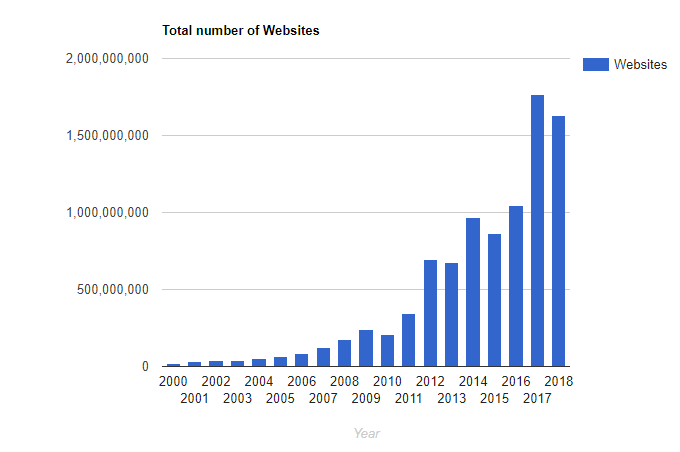
\includegraphics[width=\textwidth]{Images/numberOfWebsites.png}
    \caption{Total number of websites since 2000 (\cite{NumberofWebsites})}
    \label{Total number of websites since 2000}
\end{figure}
The majority of small businesses with a website are run by single individuals or small teams that do not necessarily have the time or resources to keep on top of their web traffic and potential attacks. The proposed application needs to account for the fact that these people will likely not have enough time to go through log files given their size. They also may not have the budget to buy solutions. It should be noted that a lot of web hosts do have automatic attack detection systems in place, as these are normally included in the cost of web hosting packages. However, many web hosts run a large number of servers, each of which often has a large volume of accounts. This can be seen in a recent article about cPanel's licensing update: Ryan Gray notes that 100 accounts in the early 2000s was a high number for one server, however now it is normal (\cite{cPanelArticle}). Due to their being more than one account on a server data would be aggregated to provide a overview of the server, therefore making some attacks harder to identify.

There are lots of different types of attack that can occur on a website. Some are easier to detect than others, for example, low bandwidth attacks are harder to detect. This was noted in 2014 by the National Research Council of Italy who say that "The problem is particularly challenging in virtue of the reduced amount of bandwidth generated by the attacks" (\cite{aiello2014line}). Therefore this implies that high bandwidth attacks are relatively easy to detect, so the focus of this dissertation will be to detect low bandwidth attacks and some other common attacks on websites that shall be discussed later. The findings will then be presented not to the server owner, but to the website owner so that they can be more informed about what is happening on their website.

The idea for this project came from when my own business website was attacked. I was fully prepared for a DDOS attack, however I found that there was an IP coming onto my site around 20 times in a minute that would then go away for a number of hours only to return some time later. The only way that I was able to detect this attack was by reading through that month's log file, which contained a few thousand lines of website logs, and comparing this to spikes in the server load. I felt that it would be helpful if there was a program to analyse the data. The only solutions out there were for large corporations, there wasn't anything for individual sites. There are also websites that monitor for suspicious IP addresses, for example https://www.abuseipdb.com/, however, as these would not take a server log file, you would need to input IP addresses one by one. Also, due to the fact the information is readily available online, the attackers know when they have been identified as a suspicious IP address and can easily change their IP address. Therefore there is a need for a solution that relies upon that background data but doesn't reveal what is known about an IP address. 

There is a vast amount of data in log files, although there are many limitations of the data held in these log files. They will record IP addresses however they can not record the location of those IP addresses. While there are tools such as google analytics that provide very detailed data on visitors to the site, these tools automatically filter out bots and do not show activity if the user generates an error. Another limitation of the log file comes from looking at the user agent field, whilst this records whether it is a bot, for example, google bot, this can be easily faked, and the log file cannot detect a fake google bot. Therefore, a fake google bot is a common form of attack (\cite{algiryage2018distinguishing}), due to the fact that the server cannot verify that it is a google bot.

The program will need to be easy to use for a non-expert website owner. Most website owners are computer literate however may not know how to access or analyse this type of data. Many website owners use content management systems (CMS). WordPress already has a lot of plugins available for security, and while these do a good job at blocking attacks in real-time and preventing invalid logins, they are not able to look at data over longer periods. The program aims to be compatible with all websites but due to the popularity of CMSs and wide variety of attack types, even websites that don't run a CMS  because of their market dominance (at time of writing, about 60\% of websites use WordPress (\cite{IsItWP})), may encounter these attacks without being aware.

\section{Proposed Work}
\label{proposed}
The work proposed is to write a piece of software, that will aid website management and detect traffic patterns that may take the form of a malicious attack. The finished software should also should include a database to store some data. During the main body of research I will debate and justify a type of software for writing the software. As part of the project I will also research and appropriate the most fitting database management system to handle my database storage. 

The literature review will include a critical analysis on current technologies to detect a variety attacks. This literature will help guide the development of the software by illuminating the gaps that exist in current technology. I will also look at whether network architecture can help to stop potential attacks. For example, services such as CloudFlare use an 'Anycast' network, wherein every server on the network has the same IP address, so that when a DDOS attack occurs they can spread the attack over many servers. The attacker cannot tell that they are not all going to the same server (\cite{CloudFlare}). CloudFlare could offer solutions to detect low bandwidth attacks as well.

I intend to develop the software using agile techniques. In other words, rather than fully writing the software first and then testing it, the software will be tested as throughout the development process. This will help to make the development time shorter as errors in the code will be fixed before the next stage of the software is written. 

\section{Aims and Objectives}
For this project I will have several aims and objectives.
\subsection{Aims}
\begin{enumerate}
    \item Develop a system that is able to identify different types of website traffic.
\end{enumerate}

\subsection{Objectives}
\begin{enumerate}
    \item Carry out a literature review and produce requirements documentation
    \begin{enumerate}
        \item Review of common attack techniques and how difficult or easy they are to detect.
        \item Review literature on how to present information to users on website data.
    \end{enumerate}
    \item Review of current protection that is available and how much data these programs release to the end user.
    \begin{enumerate}
        \item Look for attack prevention solutions for CMSs.
        \item Look for the reliability and ease of use for current attack prevention solutions.
    \end{enumerate}
    \item Produce relevant system documentation.
    \begin{enumerate}
        \item Produce relevant class diagram.
        \item Produce relevant Entity Relationship Diagrams (using crow's feet notation). 
        \item Produce relevant state transition diagram for interesting behaviour.
    \end{enumerate}
    \item Evaluate the project after completion.
    \begin{enumerate}
        \item Carry out a detailed test plan on the product.
        \item Check for usability with non-technical users.
    \end{enumerate}
    \item Abstract and introduction.
\end{enumerate}

\section{Skills}
For this project I will need several skills that I either already have and will develop or new skills that I will need to learn. Where I do not have the skill required I will consult learning tutorials and online literature in order to increase my knowledge. 

This project will require both networking and program skills. The networking skills will be important to ensure that I understand what the IP information tells us. This will need to be fed into the Java program in a way that is easy for the user to understand, and is not too big O complex due to the potential size of the data that could be submitted. 
\begin{enumerate}
\item Java 
\begin{enumerate}
    \item Java will form the main component of the project. I will therefore need to understand Java to a high enough standard to implement the program. Due to the complexities of the program using the right data structures to enable a quick response will be key to the program. 
    \item The majority of my modules have involved the use of Java. Even the modules that did not contain Java as a programming language helped me to develop a conceptual understanding of programming due to the concepts being similar across the board.
\end{enumerate}
\item SQL
\begin{enumerate}
    \item The main data for the project will be stored in a database, therefore it will be necessary to ensure that my SQL skills are up to scratch in order to store the data correctly and then the retrieval of the correct information will be crucial for this project. Some of the SQL queries may be complex in nature, for example nested queries may be needed.
    \item The module that most helped with SQL was the 'Relational Database' module, which covered the foundation of SQL databases, however SQL databases have also been used in the web modules and with Java in the 'Software Engineering Practice' module. \end{enumerate}
\item Networking Knowledge
\begin{enumerate}
    \item I have a basic understanding of networking and how networks work. I will need to learn how to apply this knowledge to detect attacks.
    \item I have gained some networking knowledge in the 'Computer Networks' module. 
    \item The majority of my working knowledge of networks, particularly the internet, came from my placement year, as I had to work with a variety of different websites and provide solutions to stop attacks. Nonetheless, my networking knowledge in identifying attacks is still limited and will need to be improved. 
\end{enumerate}
\item Time Management Skills
\begin{enumerate}
    \item As this is the largest project that I will work on during my undergraduate degree, I will need to manage my time well to ensure that I can get the work done and keep up with the other modules that I am taking this year. 
    \item I learnt a lot of time management skills in the 'Software Engineering' practical module. I will further develop these by asking my supervisor for advice early on and by researching time management techniques that work well for dissertation-style projects.
\end{enumerate}
\end{enumerate}

\section{Resources}

\subsection{Hardware}
\begin{enumerate}
    \item A PC - to write the software on.
\end{enumerate}
\subsection{Software}
\begin{enumerate}
    \item LAMP stack - a LAMP stack is needed to run websites on.
    \item Log files in the extended format
\end{enumerate}

\section{Structure and Contents of the Report}
\subsection{Report Structure}
\begin{enumerate} [topsep=0pt,itemsep=-0ex,partopsep=1ex,parsep=1pt,leftmargin=7ex,label=CH.\arabic*]
     \item Introduction
     \item Review of current detection methods for low bandwidth attacks
     \item Review of current detection methods for other types of attacks
     \item Tools and packages 
     \item Requirements Specifications
     \item Testing
     \item conclusions
\end{enumerate}

\subsection{List of Appendices}
\begin{enumerate} [label=\Alph*)]
    \item Terms of Reference
    \item Ethics form
    \item Risk Assessment
    \item ERD
\end{enumerate}
\section{Marking Scheme: Software Engineering Project }
\textbf{Overview}

\begin{enumerate} [topsep=0pt,itemsep=-0ex,partopsep=1ex,parsep=1pt,label=]
    \item Report: 60\%
\begin{enumerate}[topsep=0pt,itemsep=-1ex,partopsep=1ex,parsep=1ex,label=]
\item Abstract \& Introduction 	5\%
\item Analysis 			30\%
\item Synthesis 			30\%
\item  Evaluation \& Conclusions 	30\%
\item Presentation 			5\%
\end{enumerate}
\item Product 30\%
\begin{enumerate}[topsep=0pt,itemsep=-1ex,partopsep=1ex,parsep=1ex,label=]
\item Fitness for Purpose 		50\%
\item Build Quality 			50\%
\end{enumerate}
\item Viva 10\%
\end{enumerate}

\clearpage

\section{Project Plan}
\noindent
\rotatebox{90}{%!TeX root=TermsOfReference.tex

% A lot of the settings here are tuned to fit a landscape gantt chart into
% an A4 piece of paper.
\begin{ganttchart}[
time slot format=little-endian,
calendar week text=\currentweek,
x unit=2.4pt,
y unit chart=14pt,
y unit title=12pt,
title label font=\scriptsize,
bar top shift=.15,
bar height=0.7,
milestone label font = \small,
group label font = {\tiny\bfseries},
group inline label node/.append style=centered,
hgrid=true,vgrid={*6{draw=none},dotted},
region/.style={inline,group peaks width=2,
  group peaks height=0.25, group height=0.5,
  group top shift=0.2 ,group/.append style={fill=#1}},
milestone left shift=0,
milestone right shift=1,
ms/.style={inline,
    milestone inline label node/.append style={#1=0pt}}
]{11/9/19}{18/05/20} %<- Dates Gantt Chart runs from and to

\gantttitlecalendar{year,month,week=1}\\
% Highlight Smesters and Vactions
\ganttgroup[region=blue!10]{Sem 1}{23/9/19}{20/12/19}
\ganttgroup[region=red!50]{Christmas}{20/12/17}{1/1/18}
\ganttgroup[region=blue!50]{Sem 2}{15/1/20}{23/3/20}
\ganttgroup[region=green!25]{Easter}{26/3/20}{13/4/20}
\ganttgroup[region=blue!50]{Sem 2}{16/04/20}{27/04/20}\\

% Project Deadlines (from the slides)
\ganttmilestone[]{TOR}{28/10/19}
\ganttmilestone[ms=left]{\bfseries TOR}{28/10/19}
\ganttmilestone[ms=right]{Draft Analysis}{6/12/19}
\ganttmilestone[ms=left]{Submit}{30/4/20}
\ganttnewline[thick]

% --Tasks go here
% put in a title, a start date, end date...
\ganttbar{TOR}{23/9/19}{21/10/19}
\ganttbar[inline]{\emph{revise}}{25/10/19}{10/11/19}\\
\ganttbar{Analysis}{18/9/19}{24/11/19}\\
\ganttbar{Design}{31/10/19}{17/1/20}\\
\ganttbar{Build}{17/1/20}{17/2/20}\\
\ganttbar{Test}{20/2/20}{16/3/20}\\
\ganttmilestone[ms=right]{Build complete}{18/2/20}
\end{ganttchart}
}
%%TC:endingore %<- note use of \input{} not \include{}
\chapter{Ethics Form}
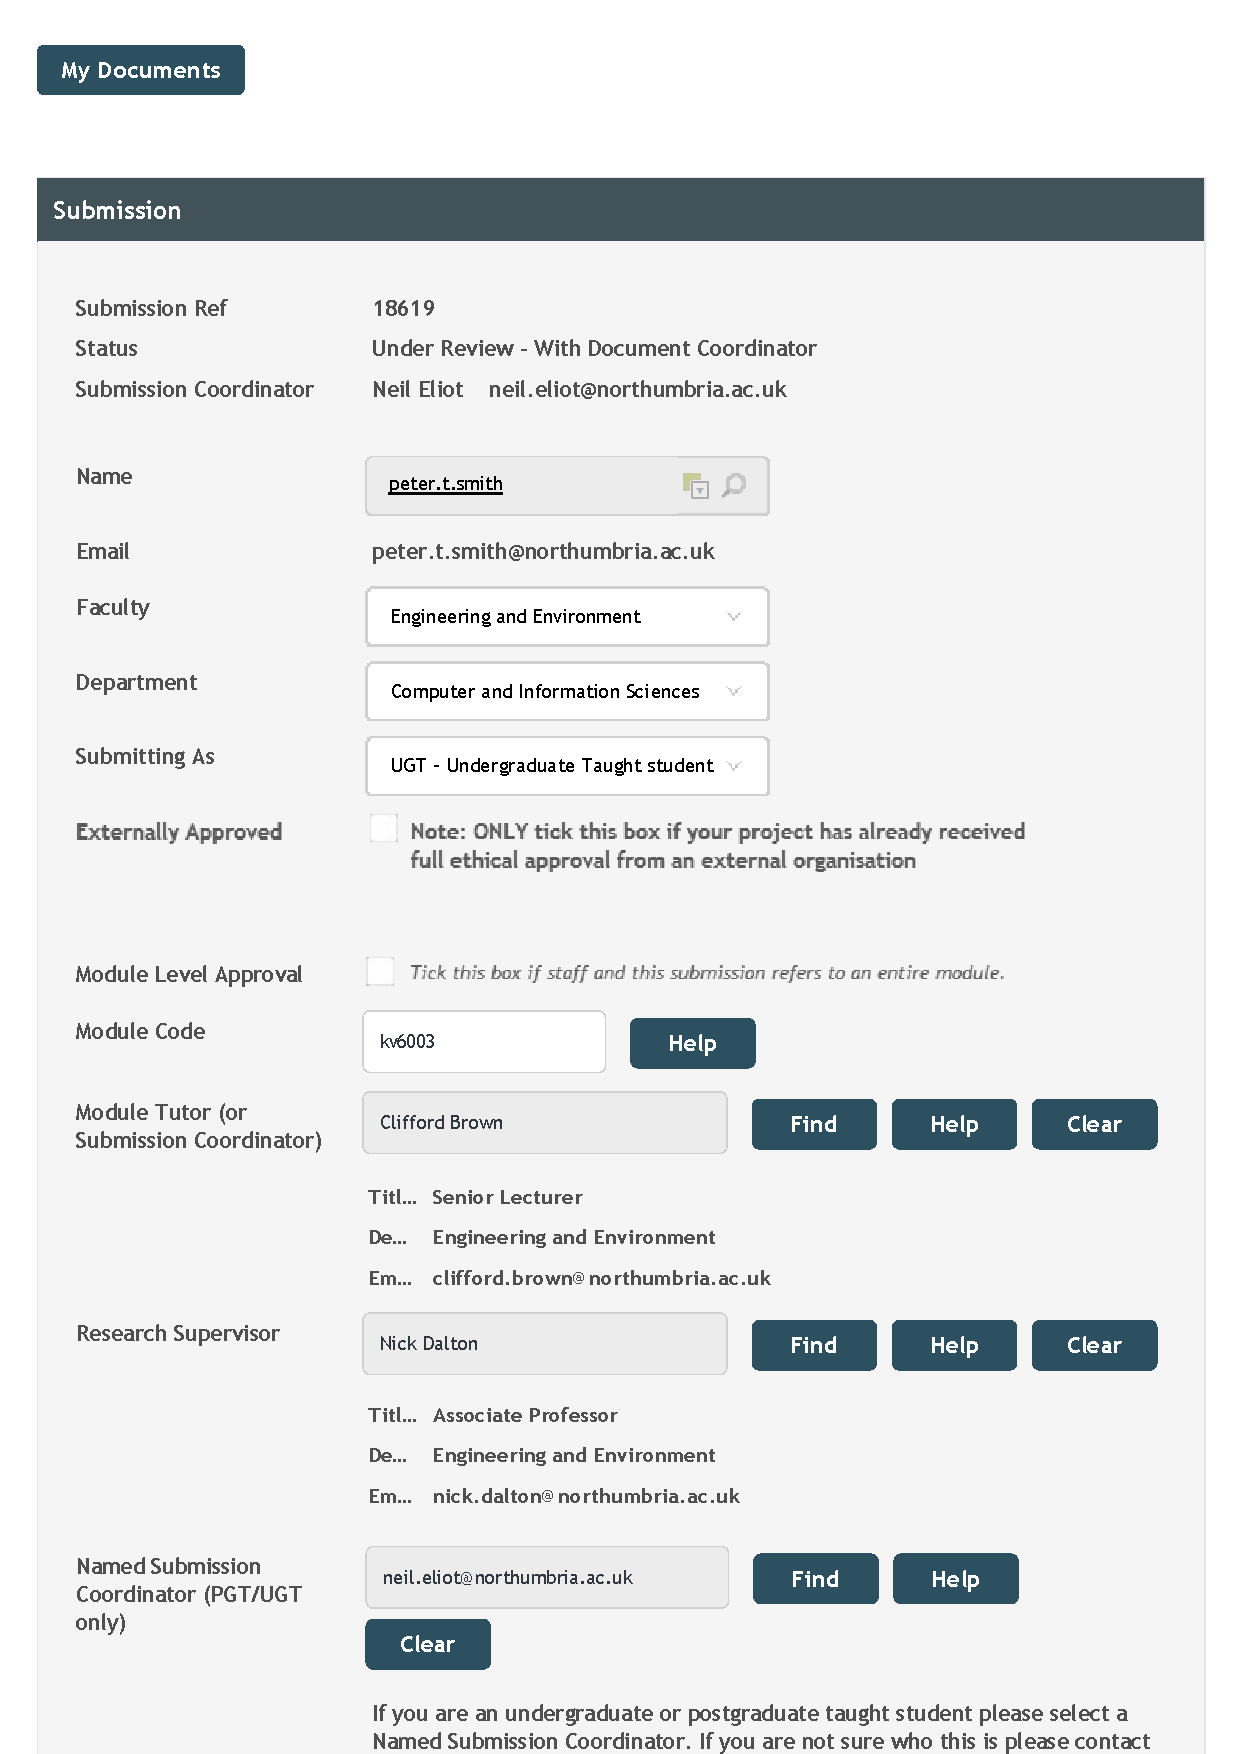
\includepdf[pages=-]{Apdenix/TermsOfReference/ResearchEthics18619.pdf}
\chapter{Participant Information Sheet}
%!TeX root=Dissertation.tex

\section{What is the purpose of this study?}
I have developed a small application to aid website owners to detect attacks on their website. This study aims to look at whether the software is usable for website owners. It is important to find out if website owners can use the software and understand the output of the data. I am conducting this study as part of my degree at Northumbria University. 
\section{Why have I been invited?}
You have invited to take part in this study as you are website owner or, you have the technical knowledge in web technology. 
\section{Do I have to take part?}
You do not have to take part in the study, you can stop at anytime. I am giving you this Participant Information Sheet to allow you to make an informed decision. You are fully able to decide whether or not you want to take part. 

\section{What will happen if I take part?}
You will be sat in front of a computer for about twenty minutes and will be asked to perform various tasks within the software. Your actions and comments will be captured using a screen recording software, you will be asked to think aloud and explain the reasons behind your actions on the software as well as what you are trying to achieve. After you have completed the task, you will be asked some general questions about your experience of using the software, this will ensure we get the same data from each participant. Your name will not be recorded on any information sheet or during the screen recording. The consent form that you will sign will not be stored with other data. On the questionnaire you will be given an I.D number which will be used to identify your recording so that we can check your questionnaire answers along with your recording. 
\section{How will my data stored and how long will it be stored for?}
Your paper consent form will be virtualised immediately upon completion and the original will be destroyed. The questionnaires will be completed online and the data will be retrieved from the online system, once all data is collected it will be deleted from the online system and stored in a password protected document on the university protected U-Drive. The videos will be stored on the university U-Drive and be destroyed after the work has been marked.  All data will be handled in accordance with the Data Protection Act (2018).
\section{What categories of personal data will be collected and processed in this study?}
Your name will be collected so that we can ensure we have your informed consent, as part of the data collection process we will be required to record your voice, this enables us to understand what users are thinking when using our software. 
\section{What is the legal basis for processing data?}
Based on the nature of the study, the data will be collected in accordance to Article 6(1)(e) "processing is necessary for the performance of a task carried out in the public interest". This study will collect a recording of your voice, due to this being sensitive personal data we will also be collecting data in accordance with Article 9 (2)(j) “processing is necessary for scientific and historical research purposes".
\section{Who are the recipients or categories of recipients of personal data, if any?}
No other external party will have access to the data provided during this study.
\section{What will happen to the results of the study and could personal data collected be used in future research?}
Once the dissertation has been marked, all personal data is deleted, any findings may be referenced in future research and the dissertation may be published.
\section{Who is Organizing and Funding the Study?}
This study is organised by Northumbria University. 
\section{Who has reviewed this study?}
The research project, submission reference 18619 has been approved in Northumbria University’s Ethics Online system. It has been reviewed in order to safeguard your interests, and have granted approval to conduct the study.
\section{What are my rights as a participant in this study?}
As a participant, you have the right to access a copy of the information collated in their personal data (to request access participants are required to submit a Subject Access Request); this can be done through email. If the participants notices that there is innacurate documentation of their personal data they have the right to request this to be corrected. You are also informed that if you are dissatisfied with the University’s processing of personal data, you have the right to complain to the Information Commissioner’s Office. 
\bigskip
\begin{center}\textbf{
    Contact for further information: }
    
Researcher Name: Peter Smith
Researcher email: peter.t.smith@northumbria.ac.uk
 
Supervisor: Nick Dalton 
Supervisor email: nick.dalton@northumbria.ac.uk

Second Marker: Neil Elliot
Second Marker email: neil.elliot@northumbria.ac.uk

Name and contact details of the Records and Information Officer at Northumbria University: Duncan James (dp.officer@northumbria.ac.uk). 

You can find out more about how we use your information at: www.northumbria.ac.uk/about-us/leadership-governance/vice-chancellors-office/legal-services-team/gdpr/gdpr---privacy-notices/ 
or by contacting a member of the research team

\end{center}
\chapter{Log file example}
\begin{figure}[H] 
    \centering
    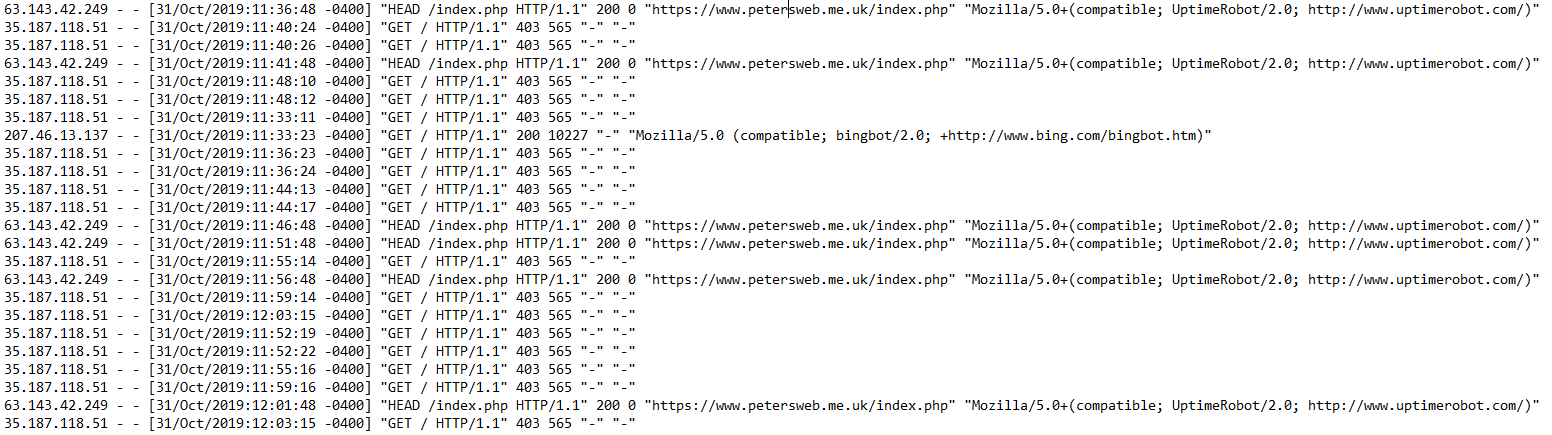
\includegraphics[width=170mm]{Apdenix/DodgyIPs.PNG}
    \caption{Log file example}
    \label{fig:my_label}
\end{figure}
\chapter{MOSCOW} \label{Moscow}
%!TeX root=Dissertation.tex

\section{Functional Requirements and Justification}
\textbf{Must}
\begin{enumerate}
    \item Allow users to analyse their website access logs.
    \begin{itemize}
        \item Users need to be able to import a large data set of website access logs, maybe a few months at a time to look for trends.
    \end{itemize}
    \item Allow users to access and view the data from their access logs.
    \begin{itemize}
        \item Users need to be able to interact with the data within the data set allowing them to make informed decisions on the data.
    \end{itemize}
    \item Use some kind of learning loop.
    \begin{itemize}
        \item Users may submit small data sets to analyse and the software needs to be able to use historical data to calculate risk. This approach could be done with the use of statistical analysis or by the use of an AI through fuzzy logic or computer learning.
    \end{itemize}
    \item Allow a admin to update known IP address'.
    \begin{itemize}
        \item An admin user needs to be able to add or remove a benign IP address' for services like google and Bing bots.
    \end{itemize}
    \item Be able to read log files.
    \begin{itemize}
        \item This will enable the detection of incoming attacks.
    \end{itemize}
        \item Allow data to be stored on an appropriate database
    \begin{itemize}
        \item For example  No SQL (MongoDB), SQL (Microsoft access)
    \end{itemize}
        \item Allow data to be stored securely in a database.
    \begin{itemize}
        \item The data that is collected needs to be stored securely in a database for future use.
    \end{itemize}
    \item Detect attacks
    \begin{itemize}
        \item The software must be able to detect a wide variety of attacks that can occur on web servers
    \end{itemize}
\end{enumerate}

\textbf{Should}
\begin{itemize}
    \item Allow users to filter data on data and time.
    \begin{itemize}
        \item Users may know a time-frame for an attack, therefore they may need to be able to narrow data down to this window.
    \end{itemize}
\end{itemize}
\textbf{Could}
\begin{itemize}
\item Be able to read log files that are in different formats.
    \begin{itemize}
        \item Consider the use of the following server types: Nginx, ISS.
    \end{itemize}
    \item Consider API integration.
    \begin{itemize}
        \item GOIPs, Abuse IPs.
    \end{itemize}
    \item Allow for concurrency in the database.
    \begin{itemize}
        \item If the software is developed further then there may be occasions when concurrency is needed within the database
    \end{itemize}
    
    \end{itemize}
\textbf{Won't}
\begin{itemize}
    \item Process the data on the server
    \begin{itemize}
        \item The only data that will be processed on the server will be the normal login or website traffic. The calculations of the formula will be processed on the PC of the person analyzing the data.
    \end{itemize}
    \item Automate the blocking of IP address' 
    \begin{itemize}
        \item Users need to maintain control of their own data, so if the program blocked IP addresses the users would not be in control. In addition to this there are a number or control panels (CPanel, plesk and custom panels) that would require custom APIs.
    \end{itemize}
\end{itemize}

\section{Non-Functional Requirements and Justification}
\textbf{Must}
\begin{itemize}
    \item Be maintainable, with well structured, commented, and documented code
    \begin{itemize}
        \item Following good practice and coding standards as well as making use of JavaDoc commenting will allow for code to be understood with greater ease, allowing for simpler maintenance and expansion of the project. 
    \end{itemize}
    \item Be able to analyse large amounts of data without draining large amounts of computational resources.
    \begin{itemize}
        \item The code shall be written to be as computationally simple as possible using the BigO notation.
    \end{itemize}
\end{itemize}
\textbf{Should}
\begin{itemize}
    \item The user interface should be aesthetically pleasing. 
    \begin{itemize}
        \item The design of the application should be easy on the eye, therefore making it easier to use.
    \end{itemize}
\end{itemize}
\textbf{Could}

\begin{itemize}
    \item Use Java for programming or find and alternative 
    \begin{itemize}
        \item Alternatives could include Python, C, PHP 
    \end{itemize}
    \item Consider making the upload facility flexible.
    \begin{itemize}
        \item There are different types of web-servers that can be used
    \end{itemize}
\end{itemize}
\textbf{Won't}\\
N/A
\chapter{Formuula Weights}
\section{Formula Weights (V.1)} \label{Weights}


The following weights are proposed for initial testing.

\begin{table}[H]
\begin{tabular}{ll}
Response Code & Weights \\
400           & +0.5    \\
401           & +5.0    \\
404           & +1.0 \\
403           & +2.0    \\
429           & +2.0    \\
500           & +0.2    \\
200           & -1.0   
\end{tabular}
\end{table}

If the URL contains 'Wp-Admin' then we shall apply an additional 3 to the risk related factor. If the URL contains 'login' in any case format an application of an additional 2 will be added to the risk factor. If the server responds with no data we shall apply an additional risk factor of 6.
\chapter{the fomula} \label{code}
\section{Code for formula}

%Python code highlighting
\label{Formula code}
\begin{lstlisting}[language=Java, caption=Formula code] 

	public double risk(String ip, DataStore dataStore, String countryCode) {
		double risk = 0;
		Database database = new Database();
		if (!database.knownBots(ip).equals("n/a")) {
			return risk;
		}
		double orrcancesOfipLog = Math
				.log(dataStore.getOrrcancesOfip().get(ip));
		orrcancesOfipLog = orrcancesOfipLog==0.00 ? 00.1 : orrcancesOfipLog;
		double countryRisk = database.countryRisk(countryCode); 
		double responseRisk = 0;
		double requestRisk = 0;
		for (Hits h : dataStore.getHits()) {
			if (h.getiPaddr().equals(ip)) {
				switch (h.getResponse()) {
				case 400:
					responseRisk += 0.5;
					break;
				case 401:
					responseRisk += 5;
					break;
				case 403:
					responseRisk += 2;
					break;
				case 404:
					responseRisk += 1;
					break;
				case 429:
					responseRisk += +2;
					break;
				case 500:
					responseRisk += 0.2;
					break;
				case 200:
					responseRisk -= 1;
					break;
				}
				if (containIgnoreCase(h.getRequest(), "wp-admin")) {
					requestRisk += 3;
				}
				if (containIgnoreCase(h.getRequest(), "login")) {
					requestRisk += 2;
				}
				if (h.getSize() == 0) {
					responseRisk = +6;
				}
			}

		}
		risk = (orrcancesOfipLog * 0.6) + ((requestRisk+responseRisk)*0.3) + (countryRisk * 0.1);
		if (risk > 100) {
			return 100;
		} else if (risk < 1) {
			return 1;
		} else {
			return risk;
		}
	}
\end{lstlisting}

\chapter{Log Book}
%!TeX root=Dissertation.tex

\TEXTBF{SEMESTER 1 WEEK 1} \\
\smallskip
\\
\begin{tabularx}{\textwidth}{|X|X|X|}
     
\hline
Date and time of meeting                         &          04/10/2019               & \begin{tabular}[c]{@{}l@{}}As scheduled:  \\Yes\end{tabular} \\ \hline
\multicolumn{3}{|l|}{Brief description of work done since last meeting:}                                                                      \\ \hline
\multicolumn{3}{|l|}{Worked on PID and TOR}                                                                                                                     \\ \hline
\multicolumn{2}{|l|}{Number of hours spent on project since last meeting:} & N/A first meeting                    \\ \hline
\multicolumn{3}{|l|}{Questions/items to discuss at meeting (agenda):}  \\ \hline 
\multicolumn{3}{|l|}{Review TOR, 
Discuss 'how to get data'}     \\ \hline
\multicolumn{3}{|l|}{Agreed tasks for next meeting:}                                                                                          \\ \hline
\multicolumn{3}{|c|}{work on tor}                                                                                                                     \\ \hline
\multicolumn{3}{|l|}{\begin{tabular}[c]{@{}l@{}}Documents discussed /any other issues:\end{tabular}}                                        \\ \hline
\multicolumn{3}{|l|}{Questions on where to get data}                                                                                                                        \\ \hline
\multicolumn{3}{|l|}{Date and time of next meeting:10/10/2019 9.30}                             \\ \hline
\end{tabularx}
\\
\smallskip
\\
%% new week
\TEXTBF{SEMESTER 1 WEEK 2} \\
\smallskip
\\
\begin{tabularx}{\textwidth}{|X|X|X|}
     
\hline
Date and time of meeting                         &          10/10/2019               & \begin{tabular}[c]{@{}l@{}}As scheduled:  \\ Yes\end{tabular} \\ \hline
\multicolumn{3}{|l|}{Brief description of work done since last meeting:}                                                                      \\ \hline
\multicolumn{3}{|l|}{Worked on TOR}                                                                                                                     \\ \hline
\multicolumn{2}{|l|}{Number of hours spent on project since last meeting:} & 5               \\ \hline
\multicolumn{3}{|l|}{Questions/items to discuss at meeting (agenda):}         \\ \hline

\multicolumn{3}{|l|}{Review TOR}     \\ \hline
\multicolumn{3}{|l|}{Agreed tasks for next meeting:}                                                                                          \\ \hline
\multicolumn{3}{|l|}{Revise TOR}                                                                                                                     \\ \hline
\multicolumn{3}{|l|}{\begin{tabular}[c]{@{}l@{}}Documents discussed/any other issues:\end{tabular}}                                        \\ \hline
\multicolumn{3}{|l|}{TOR and ethics}                                             
\\ \hline
\multicolumn{3}{|l|}{Date and time of next meeting:17/10/2019}                       \\ \hline
\end{tabularx}
\\
\smallskip
\\
\newpage
%% new week
\TEXTBF{SEMESTER 1 WEEK 3} \\
\smallskip
\\
\begin{tabularx}{\textwidth}{|X|X|X|}
     
\hline
Date and time of meeting                         &          17/10/2019               & \begin{tabular}[c]{@{}l@{}}As scheduled:  \\ Yes\end{tabular} \\ \hline
\multicolumn{3}{|l|}{Brief description of work done since last meeting:}                                                                      \\ \hline
\multicolumn{3}{|l|}{Worked on TOR}                                                                                                                     \\ \hline
\multicolumn{2}{|l|}{Number of hours spent on project since last meeting:} & 0               \\ \hline
\multicolumn{3}{|l|}{Questions/items to discuss at meeting (agenda):}         \\ \hline

\multicolumn{3}{|l|}{N/A}     \\ \hline
\multicolumn{3}{|l|}{Agreed tasks for next meeting: }     \\ \hline
\multicolumn{3}{|l|}{Revise TOR and  do ethics}                                                                                                                     \\ \hline
\multicolumn{3}{|l|}{\begin{tabular}[c]{@{}l@{}}Documents discussed/any other issues:\end{tabular}}                                        \\ \hline
\multicolumn{3}{|l|}{Looked at some code fragments}                                             
\\ \hline
\multicolumn{3}{|l|}{Date and time of next meeting:24/10/2019}                       \\ \hline
\end{tabularx}
\\
\smallskip
\\
%% new week
\TEXTBF{SEMESTER 1 WEEK 4} \\
\smallskip
\\
\begin{tabularx}{\textwidth}{|X|X|X|}
     
\hline
Date and time of meeting                         &          24/10/2019               & \begin{tabular}[c]{@{}l@{}}As scheduled:  \\ Yes\end{tabular} \\ \hline
\multicolumn{3}{|l|}{Brief description of work done since last meeting:}                                                                      \\ \hline
\multicolumn{3}{|l|}{Worked on TOR}                                                                                                                     \\ \hline
\multicolumn{2}{|l|}{Number of hours spent on project since last meeting:} & 0               \\ \hline
\multicolumn{3}{|l|}{Questions/items to discuss at meeting (agenda):}         \\ \hline

\multicolumn{3}{|l|}{N/A}     \\ \hline
\multicolumn{3}{|l|}{Agreed tasks for next meeting: }     \\ \hline
\multicolumn{3}{|l|}{Revise TOR and  do ethics}                                                                                                                     \\ \hline
\multicolumn{3}{|l|}{\begin{tabular}[c]{@{}l@{}}Documents discussed/any other issues:\end{tabular}}                                        \\ \hline
\multicolumn{3}{|l|}{Looked at Ethics forms}                                             
\\ \hline
\multicolumn{3}{|l|}{Date and time of next meeting:24/10/2019}                       \\ \hline
\end{tabularx}

%% new week
\TEXTBF{SEMESTER 1 WEEK 5} \\
\smallskip
\\
\begin{tabularx}{\textwidth}{|X|X|X|}
     
\hline
Date and time of meeting                         &          31/10/2019               & \begin{tabular}[c]{@{}l@{}}As scheduled:  \\ Yes\end{tabular} \\ \hline
\multicolumn{3}{|l|}{Brief description of work done since last meeting:}                                                                      \\ \hline
\multicolumn{3}{|l|}{Ethics and chapter 2}                                                                                                                     \\ \hline
\multicolumn{2}{|l|}{Number of hours spent on project since last meeting:} &  5               \\ \hline
\multicolumn{3}{|l|}{Questions/items to discuss at meeting (agenda):}         \\ \hline

\multicolumn{3}{|l|}{N/A}     \\ \hline
\multicolumn{3}{|l|}{Agreed tasks for next meeting: }     \\ \hline
\multicolumn{3}{|l|}{Get ethics sorted (error on forms}                                                                                                                     \\ \hline
\multicolumn{3}{|l|}{\begin{tabular}[c]{@{}l@{}}Documents discussed/any other issues:\end{tabular}}                                        \\ \hline
\multicolumn{3}{|l|}{Looked at Ethics forms}                                             
\\ \hline
\multicolumn{3}{|l|}{Date and time of next meeting:24/10/2019}                       \\ \hline
\end{tabularx}

\end{document}
